\documentclass{report}

\usepackage[utf8]{inputenc}
\usepackage[brazil]{babel}
\usepackage{mathtools}
\usepackage{graphicx}
\graphicspath{{./Imagens/}}
\usepackage{subcaption}
\usepackage{epstopdf}
\usepackage{float}
\usepackage{listings}
\usepackage{courier}
\usepackage{eqnarray}
\usepackage{amsmath}
\usepackage{amsfonts}
\usepackage[dvipsnames]{xcolor}
\usepackage{verbatim}
\usepackage{arydshln}
\setlength{\dashlinegap}{0.5pt} % Espaçamento da linha tracejada

\lstset{
	backgroundcolor=\color[rgb]{1,1,0.9},
	frame = single,
	basicstyle = \footnotesize,
	keywordstyle = \color{blue},
	commentstyle = \color[rgb]{0,0.5,0},
	stringstyle = \color{Purple},
	showstringspaces = false,
	mathescape,
	breaklines = true,
	language = Octave,
	inputencoding = utf8,
	extendedchars = true,
	literate = {ã}{{\~a}} 1
			   {é}{{\'e}} 1
			   {ç}{{\c{c}}} 1
			   {~}{{$\sim\ $}} 1
			   {ó}{{\'o}} 1
			   {á}{{\'a}} 1
			   {ú}{{\'u}} 1
			   {í}{{\'i}} 1
			   {õ}{{\~o}} 1
}

\begin{document}

	\begin{titlepage}
\begin{flushleft}

\textsc{\textbf{\LARGE Universidade Federal do Rio de Janeiro}}\\[0.5cm]
\textsc{\textbf{\LARGE COPPE}}\\[0.5cm]
\textsc{\textbf{\LARGE Programa de Engenharia Elétrica - PEE}}\\[0.5cm]
\textsc{\textbf{\LARGE Disciplina: Otimização Natural}}\\[0.5cm]
\textsc{\textbf{\LARGE Aluno: Gustavo Martins da Silva Nunes}}\\[0.5cm]
\textsc{\textbf{\LARGE Professor: José Gabriel}}\\[0.5cm]
\textsc{\textbf{\LARGE Data: 15/03/2016}}\\[6.5cm]

\end{flushleft}
\begin{center}
\textsc{\textbf{\huge Lista 1 - Resolução}}
\vfill
\end{center}
\end{titlepage}

	\section*{Questão 1}
	
	\textbf{1. Escreva um algoritmo genético simples (SAG) para minimização da função $y(x) = x^2 - 0.3cos(10 \pi x)$ no intervalo $x \in [-2, +2]$, utilizando um genótipo de representação binária com pelo menos 16 bits. Utilizando inicialização aleatória, execute cinco vezes o algoritmo. Comente sobre os resultados obtidos.}\\

	\paragraph{} Embora existam diversas vertentes de Algoritmos Evolucionários (sendo o Algoritmo Genético uma delas), elas seguem, em geral, uma mesma estrutura, que consiste em definir os seguintes elementos: Representação, Seleção de Pais, Recombinação, Mutação, Seleção de Sobreviventes, Inicialização e Condição de Parada. As definições escolhidas para cada um desses elementos, para essa questão, serão explicadas, assim como alguns comentários acerca dos resultados obtidos serão feitos mais adiante.\\
	
	\begin{itemize}
	
		\item[\textbf{1.}] \textbf{Representação}
		
		\paragraph{} A representação consiste em definir um \emph{genótipo} e \emph{fenótipo} para o problema em questão. O genótipo é uma codificação de um fenótipo, o qual, por sua vez, caracteriza uma possível solução para o problema. O motivo de se trabalhar com essa abordagem consiste no fato de que as operações de mutação e recombinação são aplicadas sobre o genótipo, como forma de se gerar novas soluções a serem analisadas (e, eventualmente, de se encontrar a solução ótima). Sabendo que o mínimo da função $y(x)$ ocorre em $x = 0$ e que, nesse problema, $x \in [-2;2]$, assumiu-se, por simplicidade, que existem somente 5 fenótipos (soluções) possíveis: $x = -2$, $x = -1$, $x = 0$, $x = 1$ e $x = 2$. Com isso, definiu-se que o genótipo de um indivíduo (uma possível solução) consiste em um vetor de 20 bits, o qual encontra-se segmentado em 5 regiões de 4 bits, conforme exposto abaixo. A região compreendida entre os genes 1 e 4 engloba os bits mais significativos, ao passo que a região dos genes 16 e 20 corresponde aos bits menos significativos.\\ 
		
		\begin{align*}
			G = [&
			\begin{array}{cccc:cccc:c:cccc}
			g_1 & g_2 & g_3 & g_4 & g_5 & g_6 & g_7 & g_8 & \cdots & 	g_{17} & g_{18} & g_{19} & g_{20}
			\end{array}
			],\\\\ 
			& onde \  g_m \in \{0, 1 \},\ m = 1, ..., 20
		\end{align*}	\\
	
		\paragraph{} A decodificação do genótipo em um fenótipo é feita da seguinte maneira: conta-se quantos bits de valor '1' encontram-se em cada segmento. Aquele que tiver a maior contagem é mapeado em um fenótipo, segundo a seguinte regra:\\
		
		\begin{itemize}
			\item[\textbf{.}] Segmento 1 $\rightarrow$ fenótipo $x = -2$
			\item[\textbf{.}] Segmento 2 $\rightarrow$ fenótipo $x = -1$
			\item[\textbf{.}] Segmento 3 $\rightarrow$ fenótipo $x = 0$
			\item[\textbf{.}] Segmento 4 $\rightarrow$ fenótipo $x = 1$
			\item[\textbf{.}] Segmento 5 $\rightarrow$ fenótipo $x = 2$
		\end{itemize}		 
	
		\paragraph{} Em caso de empate entre segmentos, a prioridade é dada ao segmento que contém os bits mais significativos. No caso excepcional em que todos os bits valem 0, o mapeamento é feito no fenótipo correspondente ao segmento 1.\\
		
		\paragraph{} Após decodificados todos os fenótipos, calcula-se, então, a aptidão (\emph{fitness}) de cada indíviduo da população. Como está sendo buscado o mínimo da função $y(x)$, definiu-se a aptidão como sendo $-\frac{1}{y(x)}$, de modo a tornar o problema de minimização em maximização. Vale ressaltar que seria possível utilizar o próprio resultado da função $y(x)$ como aptidão do indíviduo e, então, selecionar aquele que apresentasse o menor valor. No entanto, optou-se por realizar essa transformação, por parecer mais natural, ao longo das gerações, selecionar aqueles indíviduos mais aptos e excluir os menos aptos (preservando, portanto, a analogia com a teoria da evolução das espécies, a qual os Algoritmos Evolucionários tentam usar como base).\\
		
		\item[\textbf{2.}] \textbf{Seleção de Pais}
				
		\paragraph{} A seleção de pais é feita levando-se em conta a aptidão de cada indivíduo. Com isso, as chances de um indivíduo se reproduzir são proporcionais à sua aptidão. A probabilidade de se selecionar um indivíduo para reprodução é, então, calculada, dividindo-se a sua aptidão pela soma de todas as aptidões de todos os indivíduos da população. Definiu-se que a população reprodutora tem o mesmo tamanho da população total (que, no caso, consiste em 100 indivíduos) e sua montagem é feita, buscando-se manter essa proporção. Dessa forma, indivíduos mais aptos são copiados mais vezes para a população reprodutora, garantindo que eles terão mais chances de gerarem mais filhos. Para a montagem da população reprodutora, escolheu-se o algoritmo conhecido como \emph{Stochastic Universal Sampling}, exibido no código mais adiante.\\
		
		\item[\textbf{3.}] \textbf{Recombinação}
		
		\paragraph{} Com a população de reprodutores montada, começa-se a geração da população de filhos. Nesse problema, definiu-se que a quantidade de filhos gerados será igual à população (no caso, 100). Cada par de pais selecionados gera dois filhos. Os pais são sorteados aleatoriamente na população reprodutora e, uma vez selecionados, podem ou não sofrer o processo de recombinação. Caso não sofram, os filhos gerados são, simplesmente, cópias de ambos os pais.\\
		
		%\paragraph{} O processo de recombinação adotado nesse problema é conhecido como \emph{``One-point Crossover"} e consiste, basicamente, em sortear uma posição aleatória do genótipo, dividindo-o em duas regiões. A montagem dos filhos é feita, então, combinando metades distintas de cada pai (filho 1 = metade 1 do pai 1 + metade 2 do pai 2 e filho 2 = metade 1 do pai 2 + metade 2 do pai 1).\\

		\paragraph{} O processo de recombinação adotado nesse problema é conhecido como \emph{``Recombinação Uniforme"} e consiste, basicamente, para cada gene, em sortear um número aleatório da distribuição uniforme entre 0 e 1 e avaliá-lo. Caso seja maior do que 0.5, o filho 1 receberá o gene em questão do pai 1 e o filho 2, do pai 2. Caso contrário, o recebimento do gene é trocado: o filho 1 recebe o gene do pai 2, enquanto que o filho 2, do pai 1.\\
		
		\item[\textbf{4.}] \textbf{Mutação}
		
		\paragraph{} Após gerados os filhos, podem ocorrer, ainda, mutações nos genes. Para esse problema, arbitrou-se que a mutação ocorre, somente, nos filhos gerados e que o novo indivíduo gerado pela mutação substitui sua versão pré-mutação (ao invés de se preservar os indivíduos pré- e pós-mutação). A mutação consiste em trocar o valor do gene em questão. Portanto, se o gene tiver valor 1, ele muda para 0 e vice-versa.\\
		
		\item[\textbf{5.}] \textbf{Seleção de Sobreviventes}
		
		\paragraph{} Com os filhos finalizados, resta selecionar os indíviduos que seguirão para a geração seguinte. No problema em questão, a abordagem adotada foi a \emph{generacional}, a qual consiste, simplesmente, em selecionar todos os filhos gerados para compor a nova geração, descartando todos os pais.\\
		
		\item[\textbf{6.}] \textbf{Inicialização}
		
		\paragraph{} A inicialização da população é feita de forma aleatória.\\
		
		\item[\textbf{7.}] \textbf{Condição de Parada}
		
		\paragraph{} O algoritmo encerra sua execução após se atingir um determinado número de gerações.\\
	
	\end{itemize}

	\paragraph{} O código, feito em Octave, encontra-se a seguir:\\
	
	\begin{lstlisting}
clear all
close all
clc

N_pop = 10; % Tamanho da população
N_bits = 20; % Quantidade de bits por genótipo
N_exec = 5; % Quantidade de vezes que o algoritmo será executado
p_rec = 0.8; % Probabilidade de haver recombinação
p_mut = 0.05; % Probabilidade de haver mutação
N_ger = 20; % Quantidade de gerações que serão consideradas
cont_ger = zeros(1,N_exec); % Armazena em que geração o ponto ótimo foi alcançado em cada execução

for t = 1:N_exec

    P = unidrnd(2, [N_bits, N_pop]) - 1; % Inicializa aleatóriamente a população
    n = 1; % Geração atual
    y = zeros(1, N_pop); % Valores da função y para cada indivíduo
    fitness = zeros(1, N_pop); % Fitness de cada indivíduo
    max_fitness = zeros(1, N_ger); % Maior valor de fitness encontrado até então na geração n
    min_fitness = zeros(1, N_ger); % Menor valor de fitness encontrado até então na geração n
    media_fitness = zeros(1, N_ger); % Média dos fitness na geração n

    while (n <= N_ger) % Critério de parada

        %% Cálculo da função y(x) para cada indivíduo

        for i = 1:size(P,2)
            
            G = P(:,i); % Genótipo do indivíduo
            ind = 1;
            contador = zeros(1,N_bits/4); % Conta quantos 1's existem nos segmentos do genótipo

            for j = 1:(N_bits/4)

                seg = G((4*(j-1)+1):4*j);
                contador(ind) = sum(seg);
                ind = ind + 1;

            end

            if (sum(contador) == 0) % Caso do genótipo ter todos os bits 0
                seg_vencedor = N_bits/4; % Prioridade dada ao segmento dos bits menos significativos
            else
                seg_vencedor = find(contador==max(contador)); % Encontra o segmento com maior contagem de 1's
                if (size(seg_vencedor,2) > 1) % Há segmentos empatados
                    seg_vencedor = min(seg_vencedor); % Prioridade para o segmento dos bits mais significativos
                end
            end

            switch(seg_vencedor) % Decodifica o genótipo em um fenótipo x
                case 1
                    x = -2;
                case 2
                    x = -1;
                case 3
                    x = 0;
                case 4
                    x = 1;
                case 5
                    x = 2;
            end
            
            y(i) = x^2 - 0.3*cos(10*pi*x); % Calcula o valor de y para o indíviduo
            fitness(i) = - 1/y(i); % Calcula o fitness do indivíduo
        end

        min_fitness(n) = min(fitness);
        max_fitness(n) = max(fitness);
        media_fitness(n) = mean(fitness);

        %% Seleção de pais

        % Probabilidade de cada indivíduo proporcional ao fitness

        pdf_fitness = abs(fitness)/sum(abs(fitness)); % Vetor de probabilidades de cada indivíduo

        cdf_fitness = cumsum(pdf_fitness);


        % Algoritmo 'Stochastic Universal Sampling'

        i = 1;
        membro_atual = i;
        r = unifrnd(0, 1/N_pop); % Sorteia um número da distribuição uniforme entre 0 e 1/N_pop
        reprodutores = zeros(1,N_pop); % Pais que serão selecionados para reproduzir

        while (membro_atual <= N_pop)
            while (r <= cdf_fitness(i))
                reprodutores(membro_atual) = i;
                r = r + 1/N_pop;
                membro_atual = membro_atual + 1;
            end
            i = i+1;
        end

        P_new = zeros(size(P)); % Nova geração

        for i = 1:2:(size(P_new)-1)


            p1 = unidrnd(length(reprodutores)); % Seleciona o primeiro pai
            p2 = unidrnd(length(reprodutores)); % Seleciona o segundo pai
            
            while (p2 == p1)
                p2 = unidrnd(length(reprodutores)); % Evita que seja sorteado o mesmo pai
            end
            
            % Recombinação uniforme
            
            r = unifrnd(0,1); % Sorteia um número da distribuição uniforme entre 0 e 1
            if (r < p_rec) % Ocorrerá recombinação
                for j = 1:N_bits
                    q = unifrnd(0,1); % Sorteia um número da distribuição uniforme entre 0 e 1
                    if (r > 0.5) 
                        P_new(j,i) = P(j, reprodutores(p1)); % Filho 1 recebe gene j do pai 1
                        P_new(j,(i+1)) = P(j, reprodutores(p2)); % Filho 2 recebe gene j do pai 2
                    else
                        P_new(j,i) = P(j, reprodutores(p2)); % Filho 1 recebe gene j do pai 2
                        P_new(j,(i+1)) = P(j, reprodutores(p1)); % Filho 2 recebe gene j do pai 1
                    end
                end
            else
                P_new(:,i) = P(:,reprodutores(p1));
                P_new(:,(i+1)) = P(:,reprodutores(p2));
            end

        end
        
        % Mutação bit a bit
        
        for j = 1:size(P_new,2)
            for k = 1:size(P_new,1)
                r = unifrnd(0,1); 
                if (r < p_mut) % Ocorrerá mutação
                    if (P_new(k,j) == 1)
                        P_new(k,j) = 0; % Comuta o bit
                    else
                        P_new(k,j) = 1; % Comuta o bit
                    end
                end
            end
        end

        % Seleção dos sobreviventes

        P = P_new; % Seleção Generacional
        n = n + 1;
    end

   cont_ger(t) = find(max_fitness == max(max_fitness),1);

end

	\end{lstlisting}
	
	\paragraph{} Em virtude da representação escolhida, o algoritmo alcança o valor ótimo bem rapidamente. Na realidade, em muitas das vezes, a solução ótima já se encontra na primeira geração, a qual é obtida através de uma inicialização aleatória da população. Essa foi uma das justificativas de se utilizar como critério de parada somente um número fixo de gerações, em vez de incluir, também, a obtenção da solução ótima e isso permite analisar como se caracterizam as populações de cada geração. Por conta disso, também escolheu-se uma população bastante reduzida (20 indivíduos), como forma de se tentar diminuir as chances de se obter logo na primeira geração a solução ótima. Em 4 das 5 vezes que o algoritmo foi executado, o ótimo global foi alcançado logo na primeira geração, ao passo que na 5ª vez, foram precisas 4 gerações até que ele fosse encontrado.\\ 
	
	\paragraph{} A Figura \ref{melhores_fitness} mostra o valor da melhor aptidão encontrada em cada geração, no caso dessa última execução (lembrando que o valor mínimo de $y(x) = -0.3$ resulta em uma aptidão de $-\frac{1}{y(x)} = \frac{10}{3} \approx 3.33$). Note que após a 4ª geração, quando o ótimo é encontrado, a solução ótima se preserva. Além disso, mais indivíduos que representam essa solução começam a fazer parte das populações subsequentes, conforme se observa na Figura \ref{media_fitness}, de modo que, a partir da 8ª geração, eles começam a dominar a população. Esse é um comportamento que se observa nas demais execuções do programa e reflete o fato de que os indivíduos mais aptos têm mais chances de se reproduzir e, consequentemente, de gerar filhos também mais aptos. Ao mesmo tempo, o critério adotado para a seleção de pais permite que, eventualmente, indíviduos menos aptos se reproduzam e gerem filhos menos aptos, conforme se nota na última geração da Figura \ref{media_fitness}. A tendência, no entanto, é que os indivíduos de melhor aptidão dominem completamente a população.\\
	
	\begin{figure}[H]
		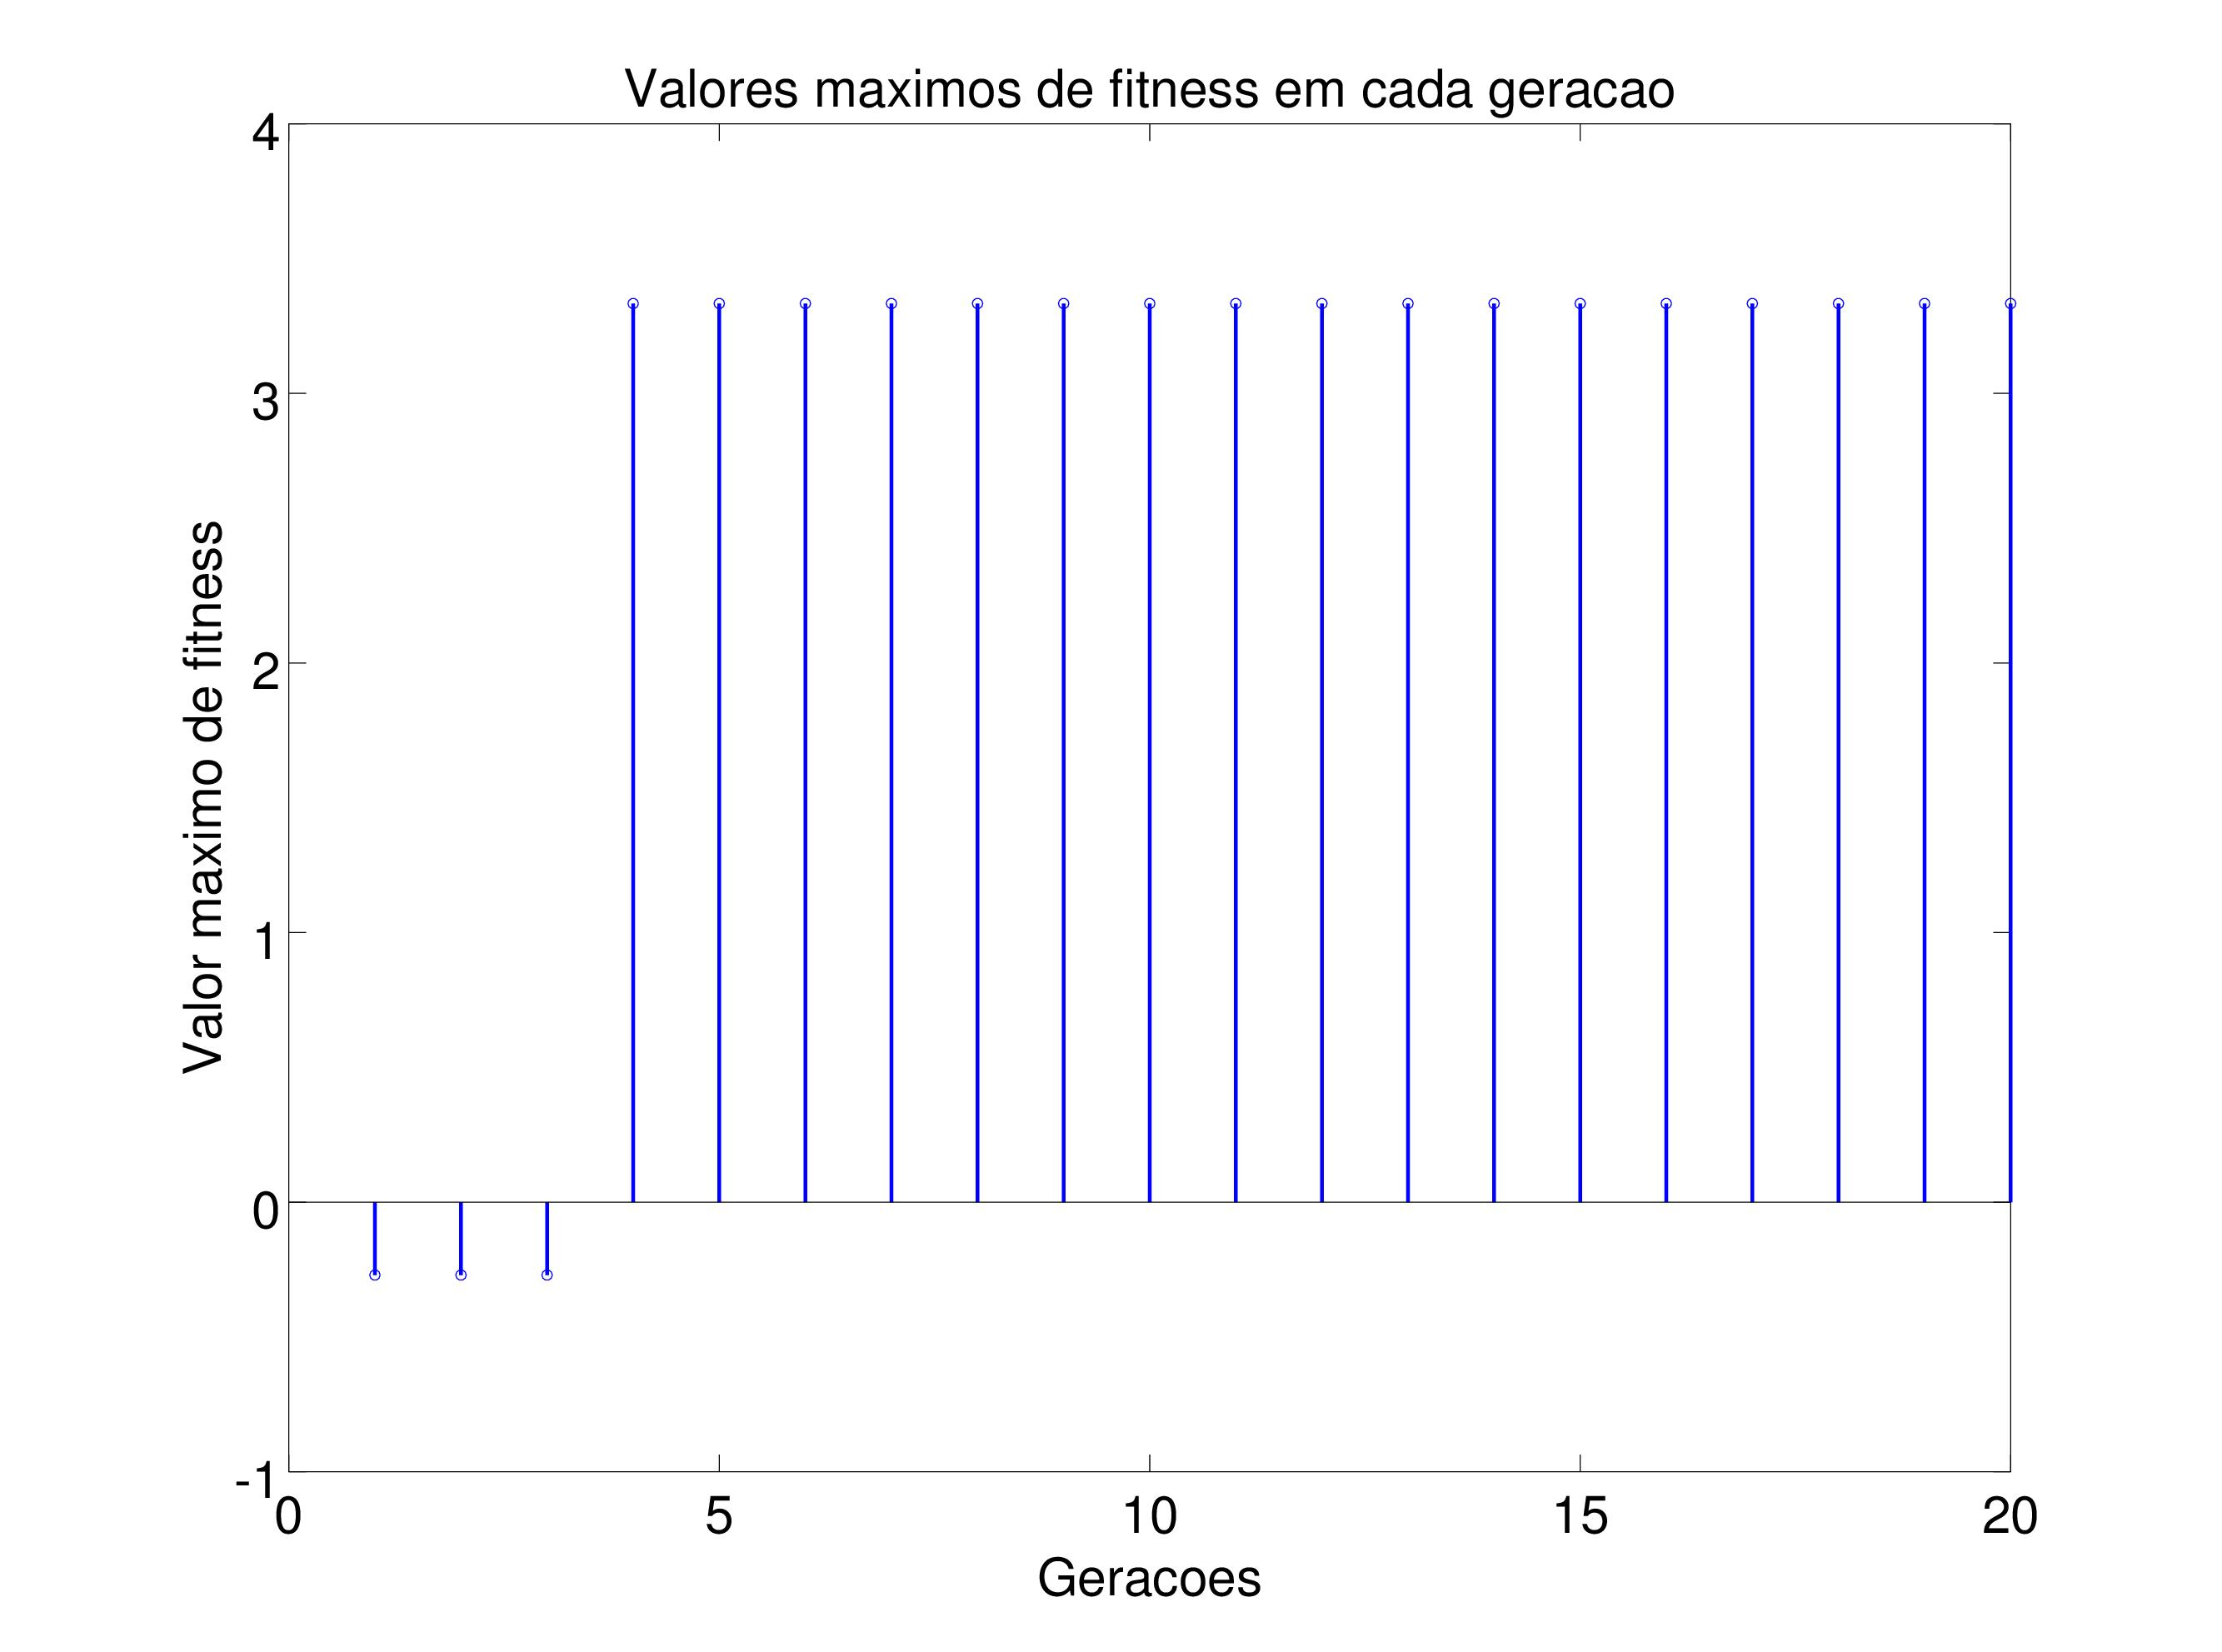
\includegraphics[width=0.9\textwidth]{Q01_melhores_fitness.jpg}
		\caption{Melhores aptidões encontradas ao longo das gerações}
		\label{melhores_fitness}
	\end{figure}
	
	\begin{figure}[H]
		\centering
		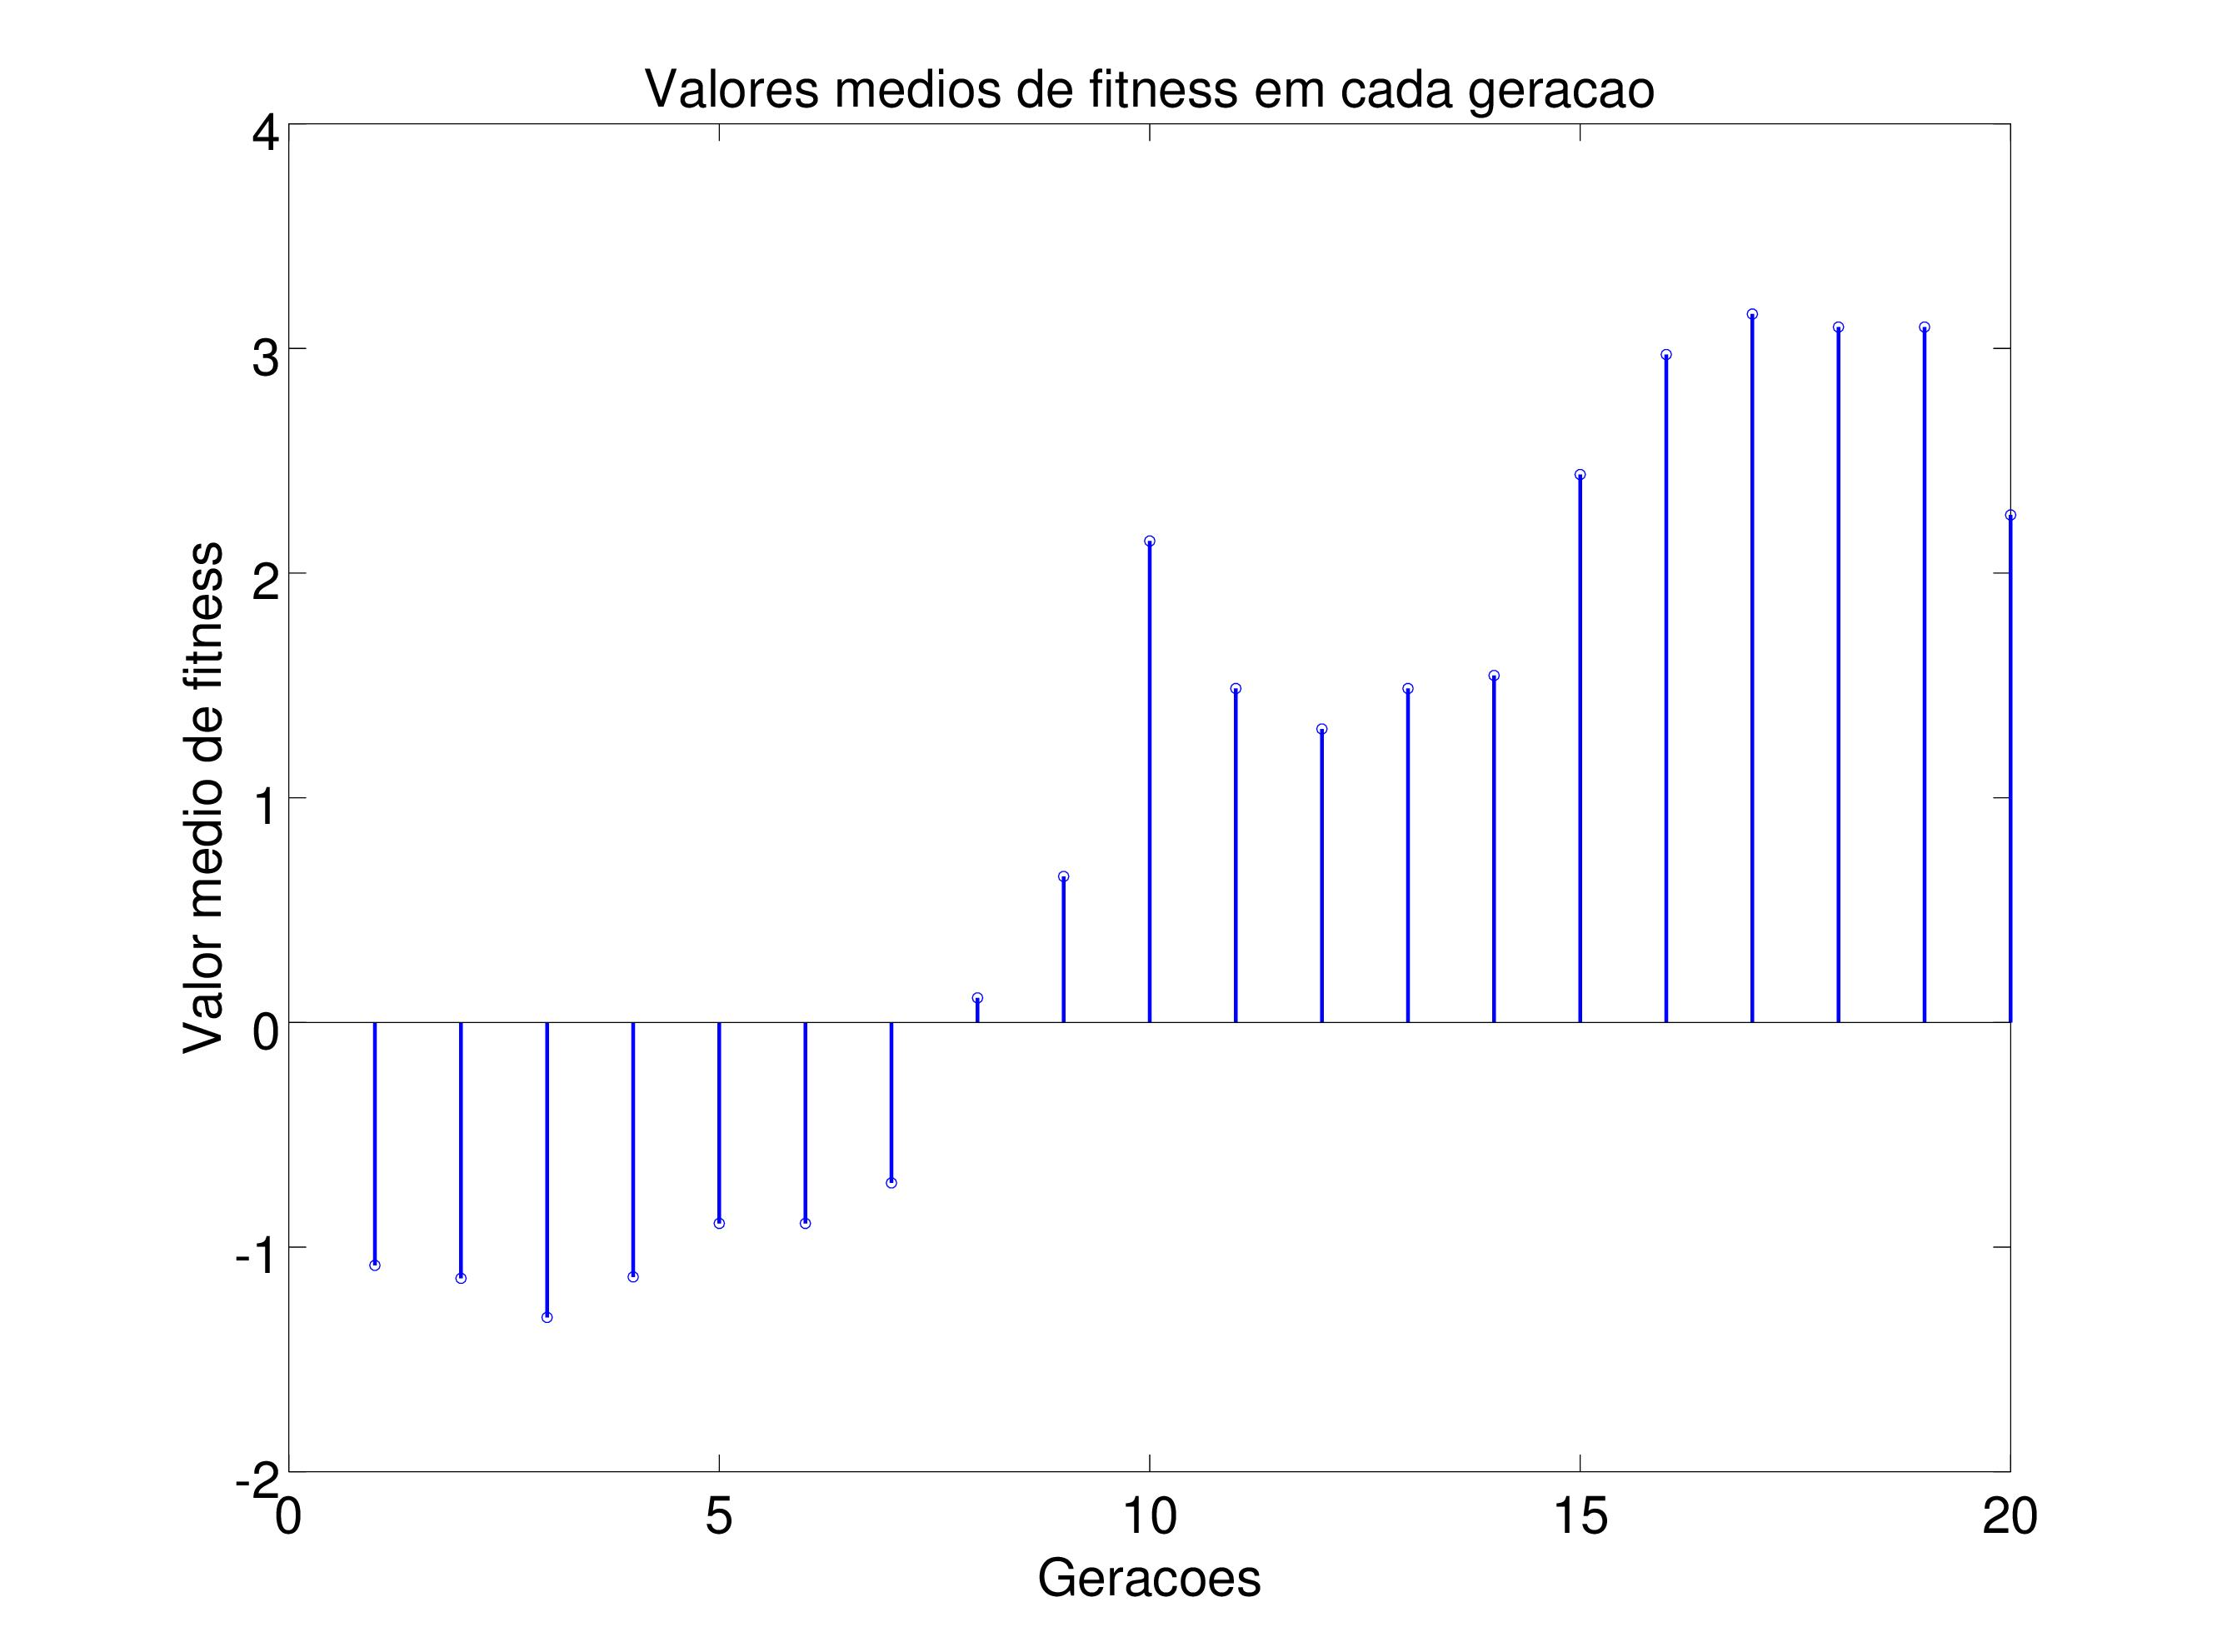
\includegraphics[width=0.9\textwidth]{Q01_media_fitness.jpg}
		\caption{Valores médios de aptidões encontrados ao longo das gerações}
		\label{media_fitness}
	\end{figure}
	
	\paragraph{} A Figura \ref{piores_fitness} exibe os menores valores encontrados de aptidão ao longo das gerações. Isso mostra que, embora os indivíduos de melhor aptidão sejam maioria nas últimas gerações, eles ainda não dominaram completamente a população (indicando que o algoritmo ainda não convergiu para a solução ótima). Vale ressaltar, também, que em gerações avançadas, quando a maioria da população corresponder a soluções ótimas, o processo de mutação tem um efeito mais ``degenerativo", uma vez que ela tenderá a tornar indivíduos com aptidão máximo em indivíduos com aptidão inferior.\\
	
	\begin{figure}[H]
		\centering
		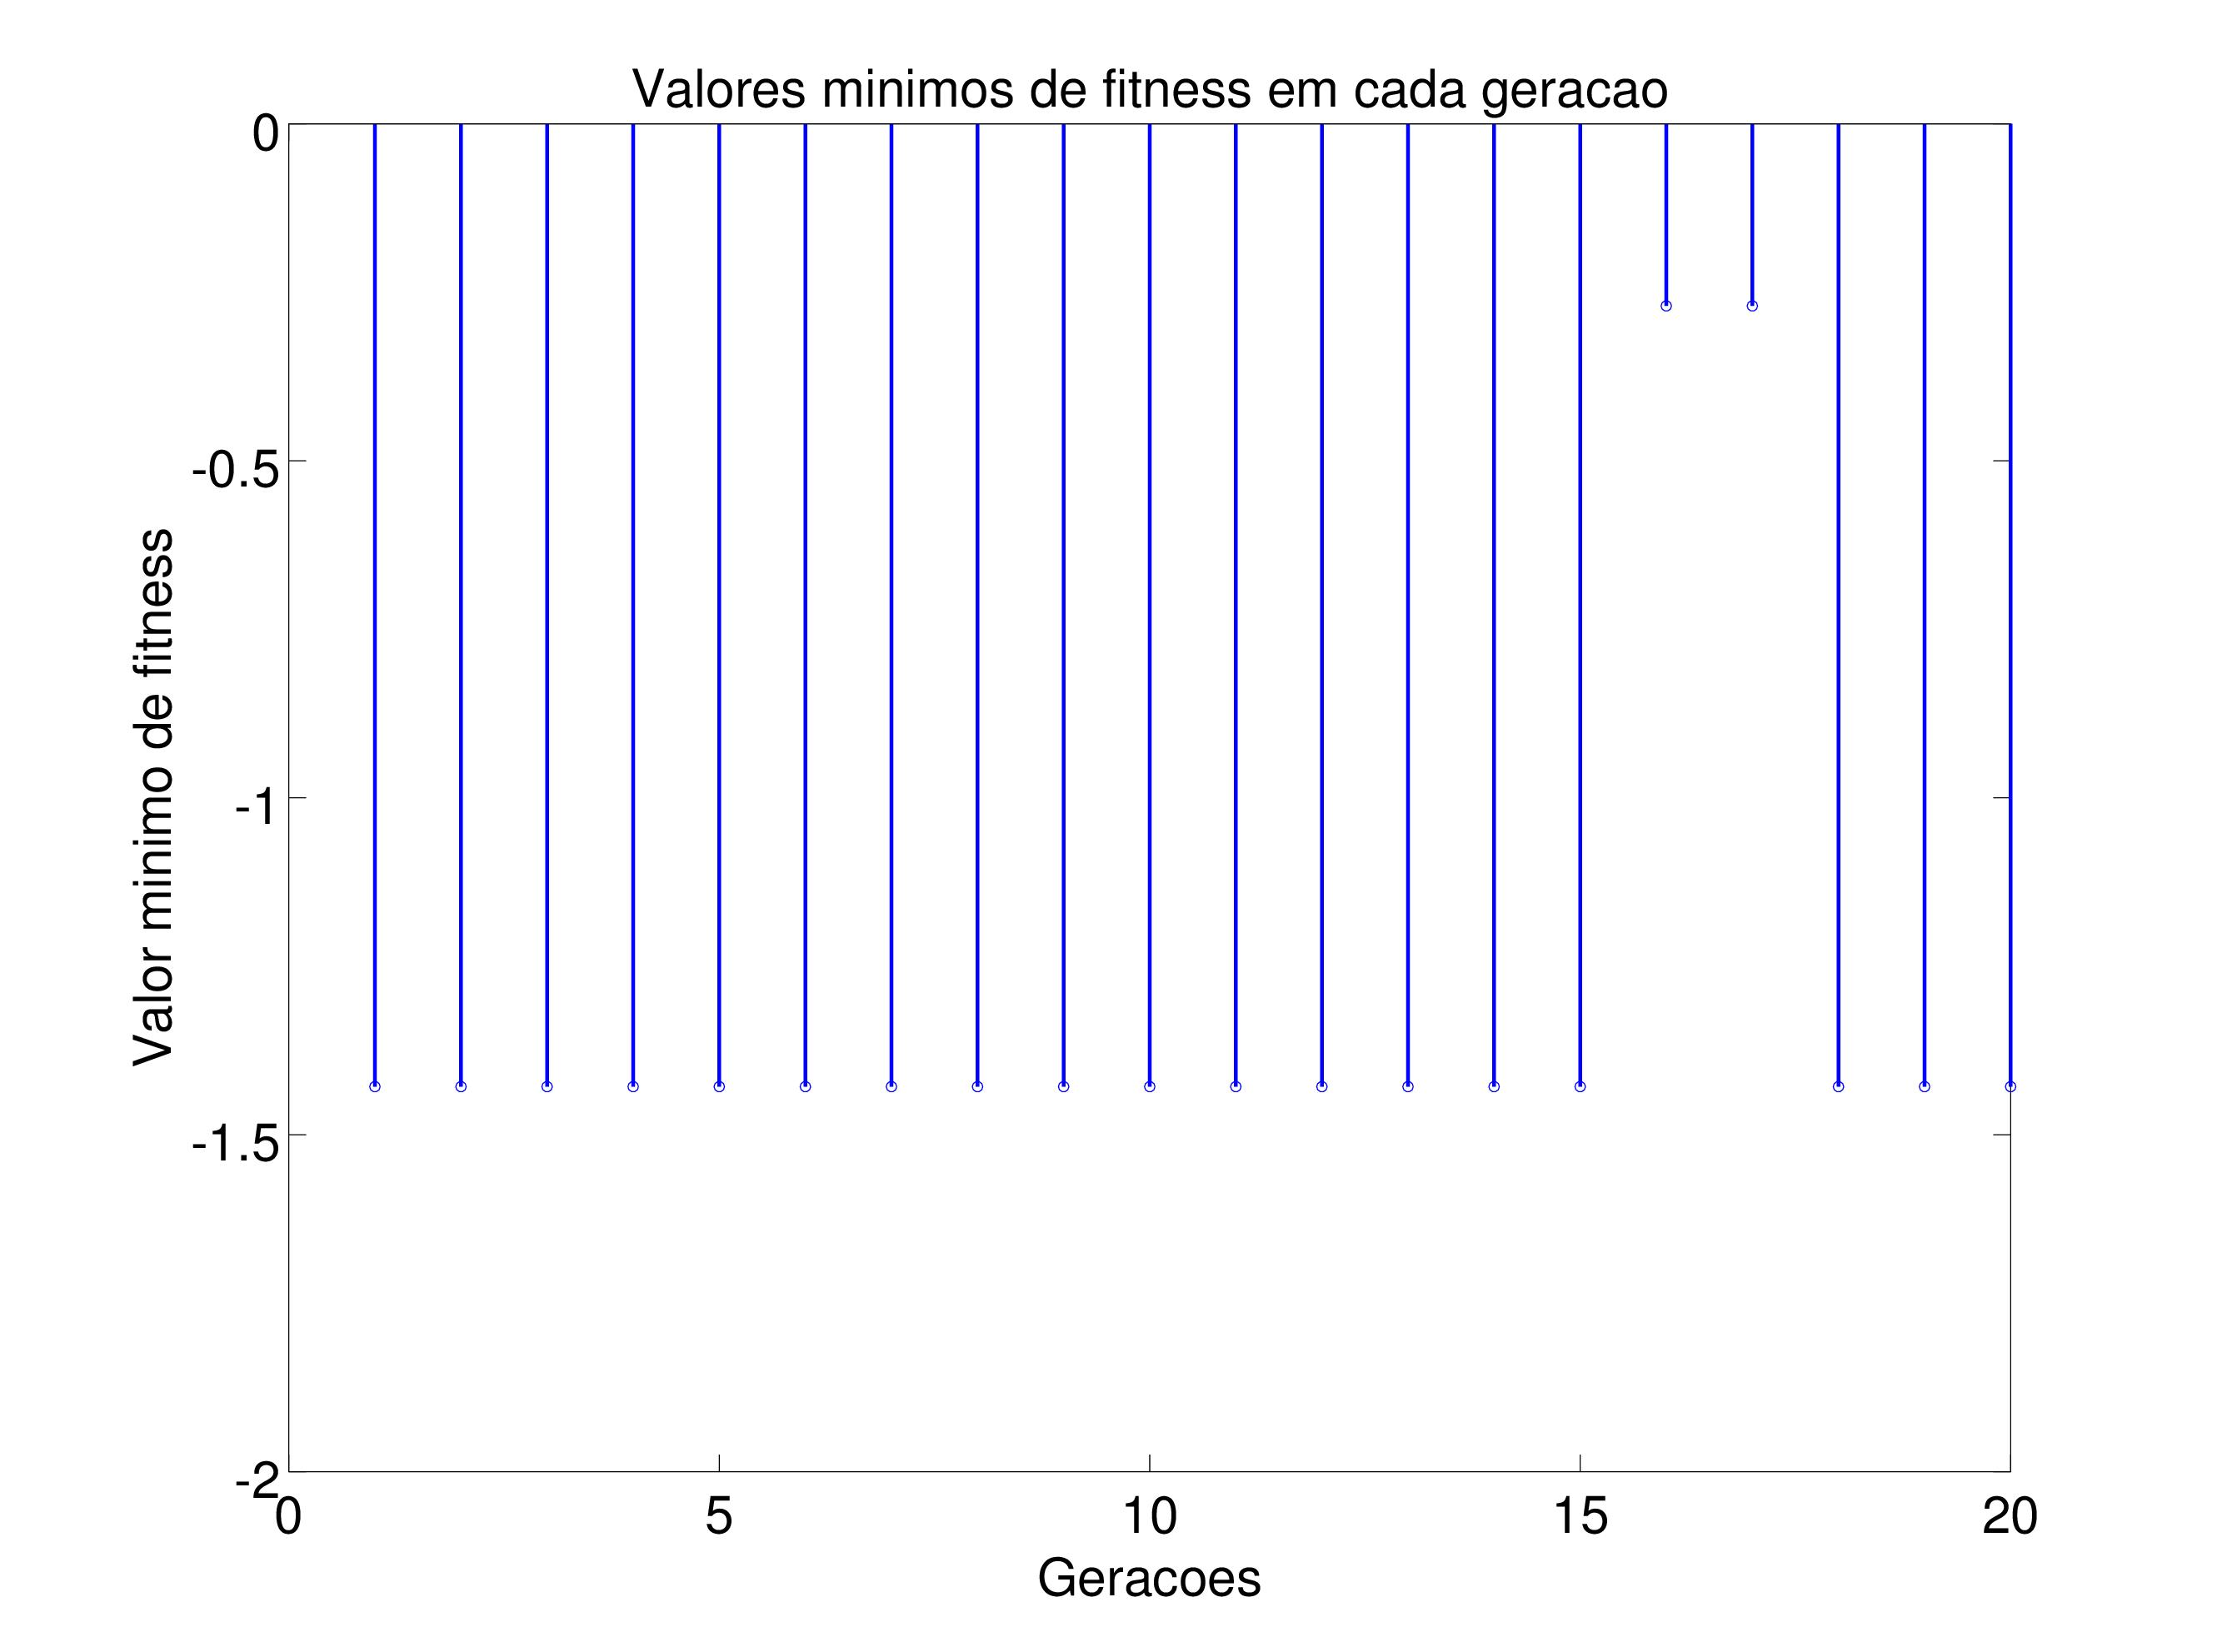
\includegraphics[width=\textwidth]{Q01_piores_fitness.jpg}
		\caption{Piores aptidões encontradas ao longo das gerações}
		\label{piores_fitness}
	\end{figure}

	\section*{Questão 2}
	
	\textbf{\textit{2. Capítulo 3, Exercício 7:}}\\\\
	\textbf{Write a computer program to implement a generational GA for the One-Max problem $f(x) = \sum_{i = 1}^{L} x_i$ (see Appendix B) with the following parameters:}\\
	\begin{itemize}
		\item \textbf{Representation: binary strings of length $L = 25$}
		\item \textbf{Initialisation: random}
		\item \textbf{Parent selection: fitness proportionate, implemented via roulette wheel or SUS}
		\item \textbf{Recombination: one-point crossover with probability $p_c = 0.7$}
		\item \textbf{Mutation: bit-flip with probability $p_m = 1/L$}
		\item \textbf{Replacement: strict generational (no elitism)}
		\item \textbf{Population size = 100}
		\item \textbf{Termination criterion: 100 generations or optimum found (whichever quickest)}
	\end{itemize}
	
	\textbf{After every generation find the best, worst, and mean fitness in the population, and plot these on a graph with the time as the $x$-axis. Now do ten runs and find the mean and standard deviation of the time taken to find the optimum.}\\
	
	\paragraph{} O código, implementado em Octave, correspondente à solução desse problema, é exibido a seguir:\\
	
	\begin{lstlisting}
Npop = 100; % Tamanho da população
L = 25; % Tamanho do genótipo
p_mut = 1/L; % Probabilidade de mutação
p_rec = 0.7; % Probabilidade de recombinação
Nger = 100; % Número máximo de gerações
n = 1; % Geração atual
T = 10; % Quantidade de rodadas do algoritmo

geracoes_otimas = zeros(1,T); % Guarda em que gerações alcançou-se o máximo de fitness

for t=1:T

    fitness = zeros(1,Npop); % Vetor de fitness da população
    max_fitness = zeros(1,Nger); % Vetor com a melhor fitness encontrada em cada geração
    min_fitness = zeros(1,Nger); % Vetor com a pior fitness encontrada em cada geração
    media_fitness = zeros(1,Nger); % Vetor com a média das fitness encontrada em cada geração

    P = unidrnd(2, [L, Npop]) - 1; % Inicialização aleatória da população

    while (n <= Nger) && (max_fitness(n) ~= 25) % Valor máximo de fitness é 25
        
        %% Cálculo de fitness
        
        fitness(n,:) = sum(P,1); % Cálculo das fitness de cada indivíduo

        max_fitness(n) = max(fitness(n,:));
        min_fitness(n) = min(fitness(n,:));
        media_fitness(n) = mean(fitness(n,:));

        %% Seleção de pais

        % Probabilidade proporcional ao fitness

        pdf_fitness = fitness/sum(fitness);
        cdf_fitness = cumsum(pdf_fitness);
        
        % Algoritmo SUS

        i = 1;
        membro_atual = i;
        r = unifrnd(0, 1/Npop);    
        reprodutores = zeros(1,Npop);

        while (membro_atual <= Npop)
            while (r <= cdf_fitness(i))
                reprodutores(membro_atual) = i;
                r = r + 1/Npop;
                membro_atual = membro_atual + 1; 
            end
            i = i + 1;
        end

        % Reprodução

        P_new = zeros(size(P)); % Nova geração

        for i = 1:2:(size(P,2) - 1)
            
            p1 = unidrnd(length(reprodutores));
            p2 = unidrnd(length(reprodutores));

            while (p2 == p1)
                p2 = unidrnd(length(reprodutores)); % Evita que a mesma posição do vetor de reprodutores seja sorteada
            end

            r = unifrnd(0,1);
            
            if (r < p_rec) % Haverá recombinação
                c = unidrnd(19); % Define o ponto de corte para recombinação
                
                P_new(1:c, i) = P(1:c, reprodutores(p1));
                P_new((c+1):end, i) = P((c+1):end, reprodutores(p2));
                P_new(1:c, (i+1)) = P(1:c, reprodutores(p2));
                P_new((c+1):end, (i+1)) = P((c+1):end, reprodutores(p2));

            else % Os pais serão somente copiados para a geração seguinte
                
                P_new(:, i) = P(:, reprodutores(p1));
                P_new(:, (i+1)) = P(:, reprodutores(p2));

            end
        end

        % Mutação bit a bit

        for j = 1:size(P_new, 2)
            for i = 1:size(P_new, 1)
                r = unifrnd(0,1);
                
                if (r < p_mut) % Haverá mutação
                    if P_new(i,j) == 0
                        P_new(i,j) = 1;
                    else
                        P_new(i,j) = 0;
                    end
                end
            end
        end

        %% Seleção dos sobreviventes    

        P = P_new; % Seleção Generacional
        n = n + 1;
    end

    if (n < Nger)
        max_fitness = max_fitness(1:n);
        min_fitness = min_fitness(1:n);
        media_fitness = media_fitness(1:n);
    end
    
    if (t == 1)
        % Plot dos gráficos

        stem(max_fitness);
        xlabel('Geração', 'FontSize', 30);
        ylabel('Fitness Máxima', 'FontSize', 30);
        title('Melhores fitness por geração', 'FontSize', 30);
        set(gca, 'FontSize', 30);
        figure;

        stem(min_fitness);
        xlabel('Geração', 'FontSize', 30);
        ylabel('Fitness Mínima', 'FontSize', 30);
        title('Piores fitness por geração', 'FontSize', 30);
        set(gca, 'FontSize', 30);
        figure;

        stem(media_fitness);
        xlabel('Geração', 'FontSize', 30);
        ylabel('Média Fitness', 'FontSize', 30);
        title('Média dos fitness por geração', 'FontSize', 30);
        set(gca, 'FontSize', 30);
    end

    geracoes_otimas(t) = n-1;

end

disp(['Média de gerações para alcançar o máximo: ' num2str(mean(geracoes_otimas))])
disp(['Desvio-padrão de gerações para alcançar o máximo: ' num2str(std(geracoes_otimas, 1))])
	\end{lstlisting}
	
	\paragraph{} As Figuras \ref{melhores_fitness_100_q02}, \ref{piores_fitness_100_q02} e \ref{media_fitness_100_q02} mostram, respectivamente, as melhores, piores e a média das fitness encontradas ao longo das gerações, em uma das execuções do programa. Conforme se observa na Figura \ref{melhores_fitness_100_q02}, a melhor fitness (correspondente ao valor $L = 25$) nunca foi alcançada. Esse fato se observou em todas as execuções do algoritmo (10 vezes), isto é, em nenhuma delas o máximo global foi alcançado. Entretanto, analisando o gráfico da Figura \ref{media_fitness_100_q02}, nota-se uma tendência de melhora das fitness da população, ao longo das gerações. Isso sugere, novamente, que indivíduos mais aptos estão dominando as populações de gerações mais recentes e que, caso se utilize mais gerações, indivíduos que representam a solução ótima virão a ser gerados.\\
	
	\begin{figure}[H]
		\centering
		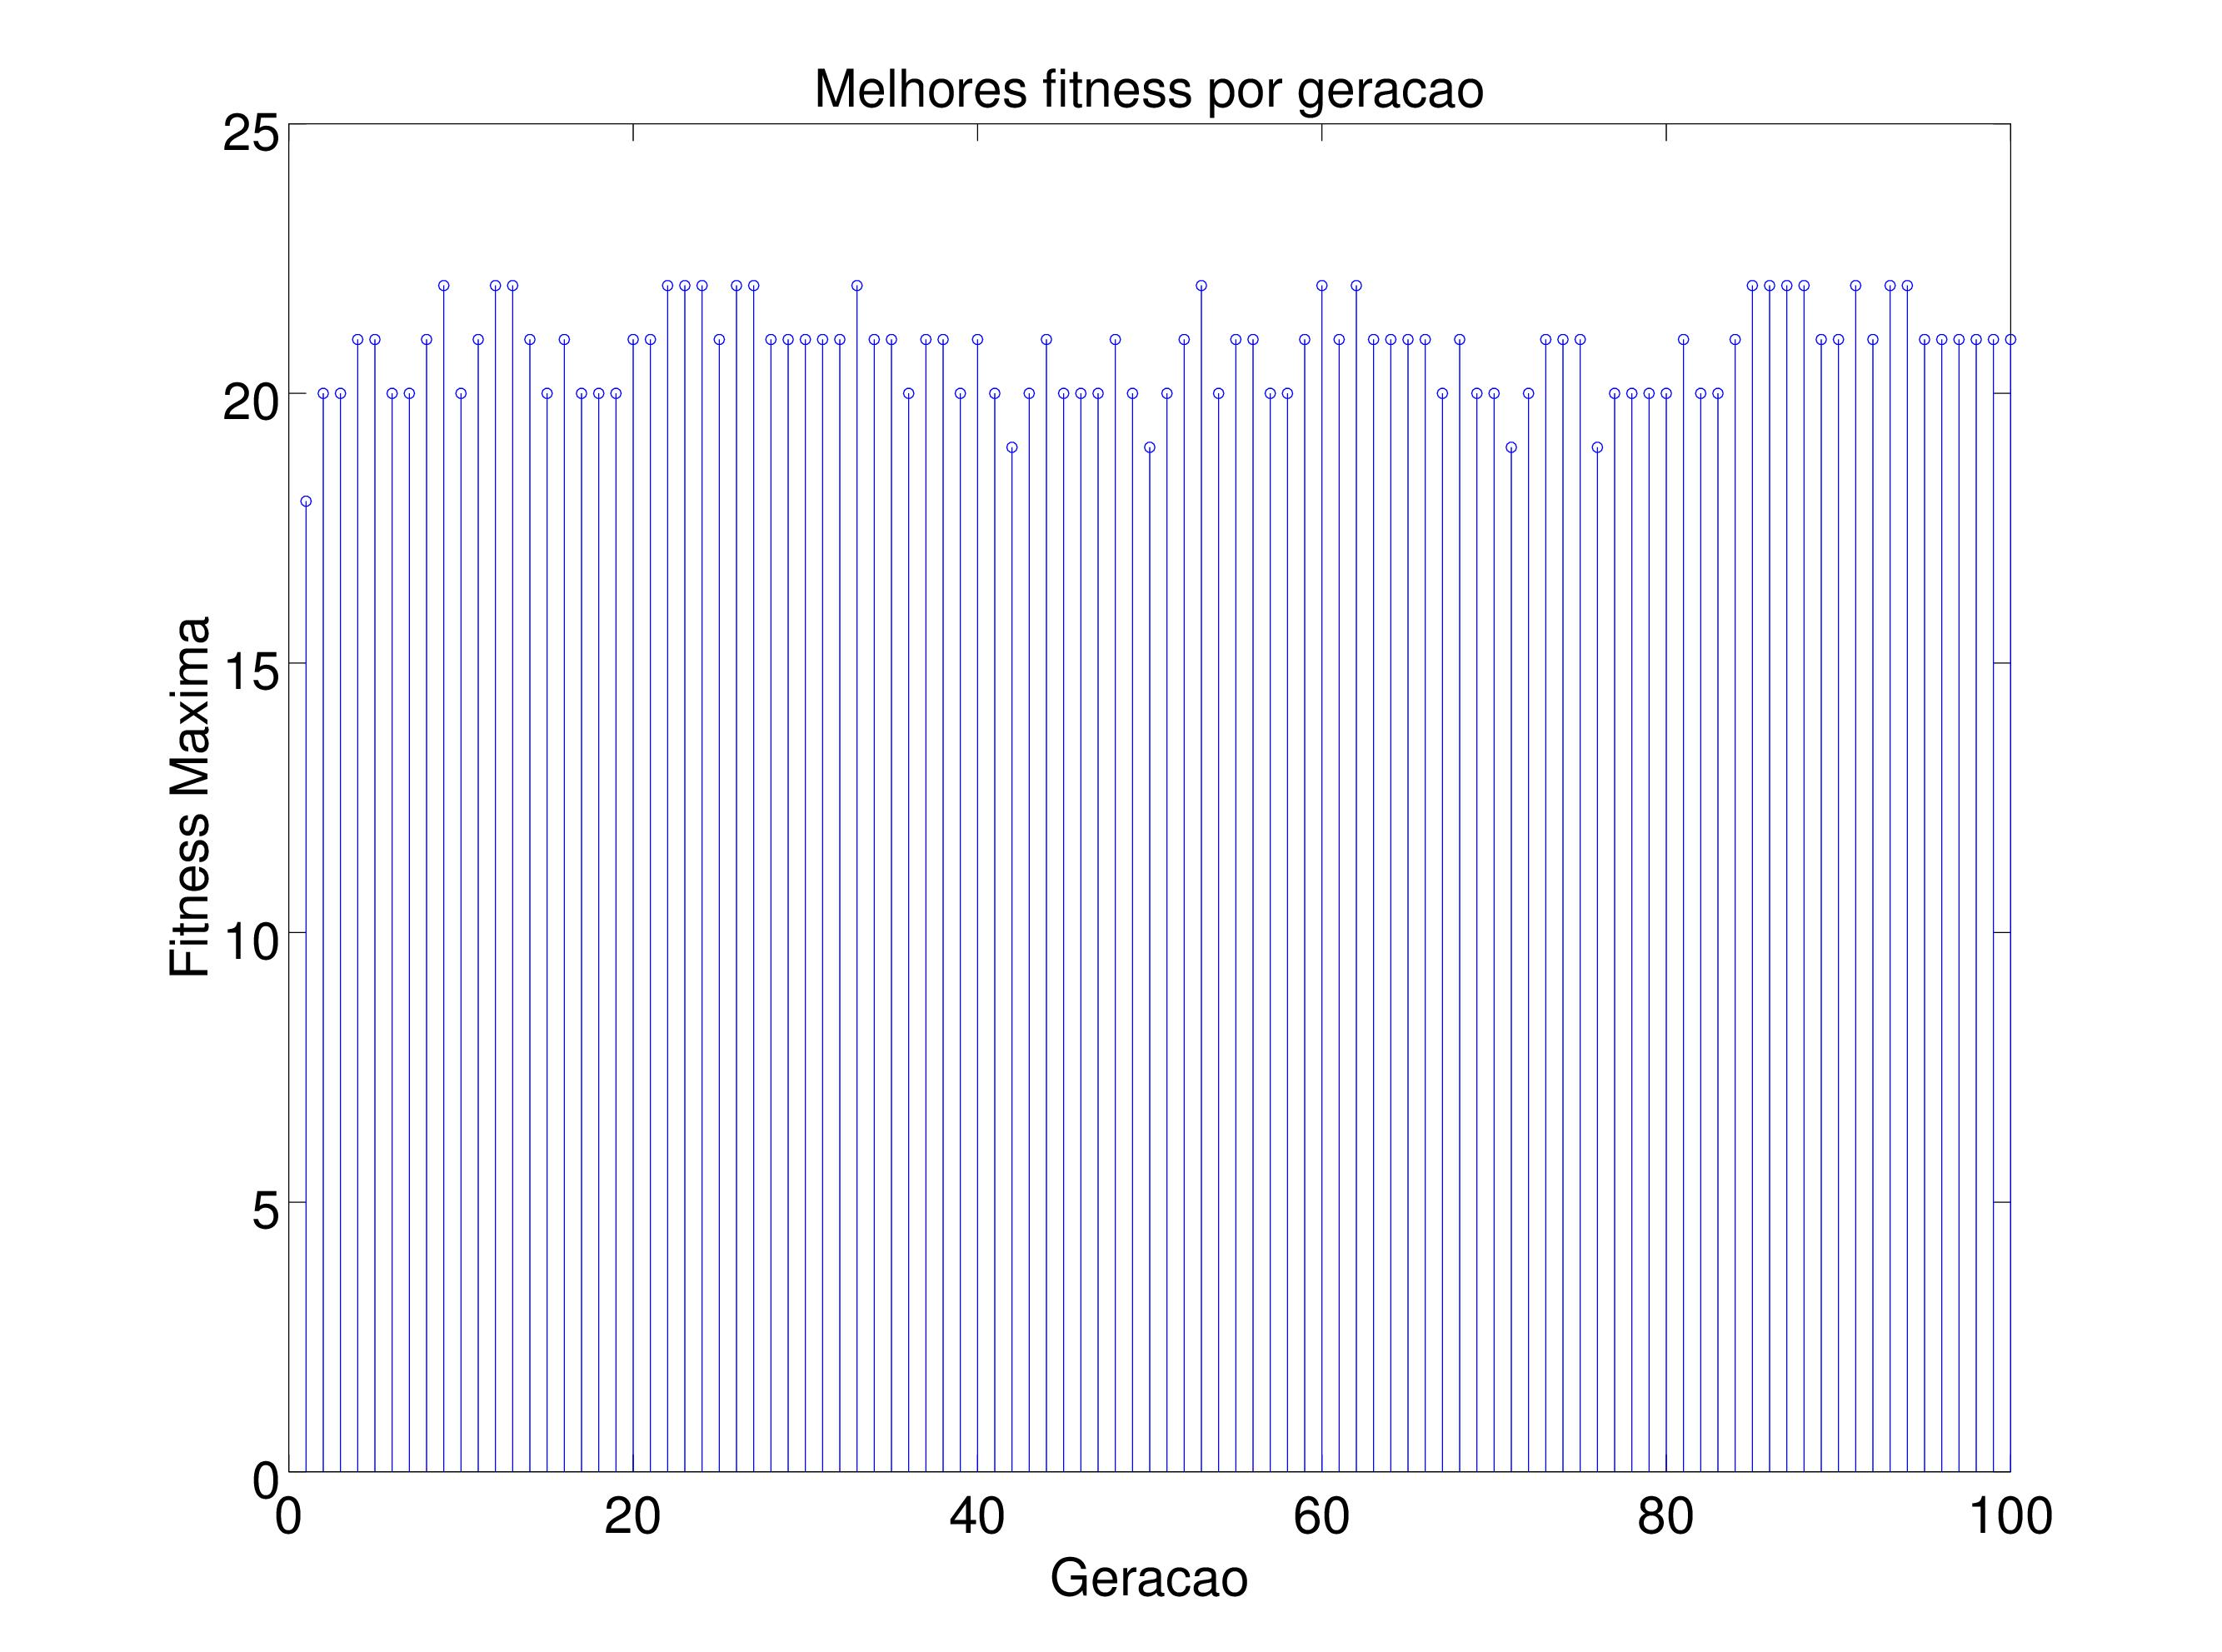
\includegraphics[width = 0.9\textwidth]{Q02_melhores_fitness_100.jpg}
		\caption{Melhores fitness encontradas ao longo de 100 gerações}
		\label{melhores_fitness_100_q02}
	\end{figure}
	
	\begin{figure}[H]
		\centering
		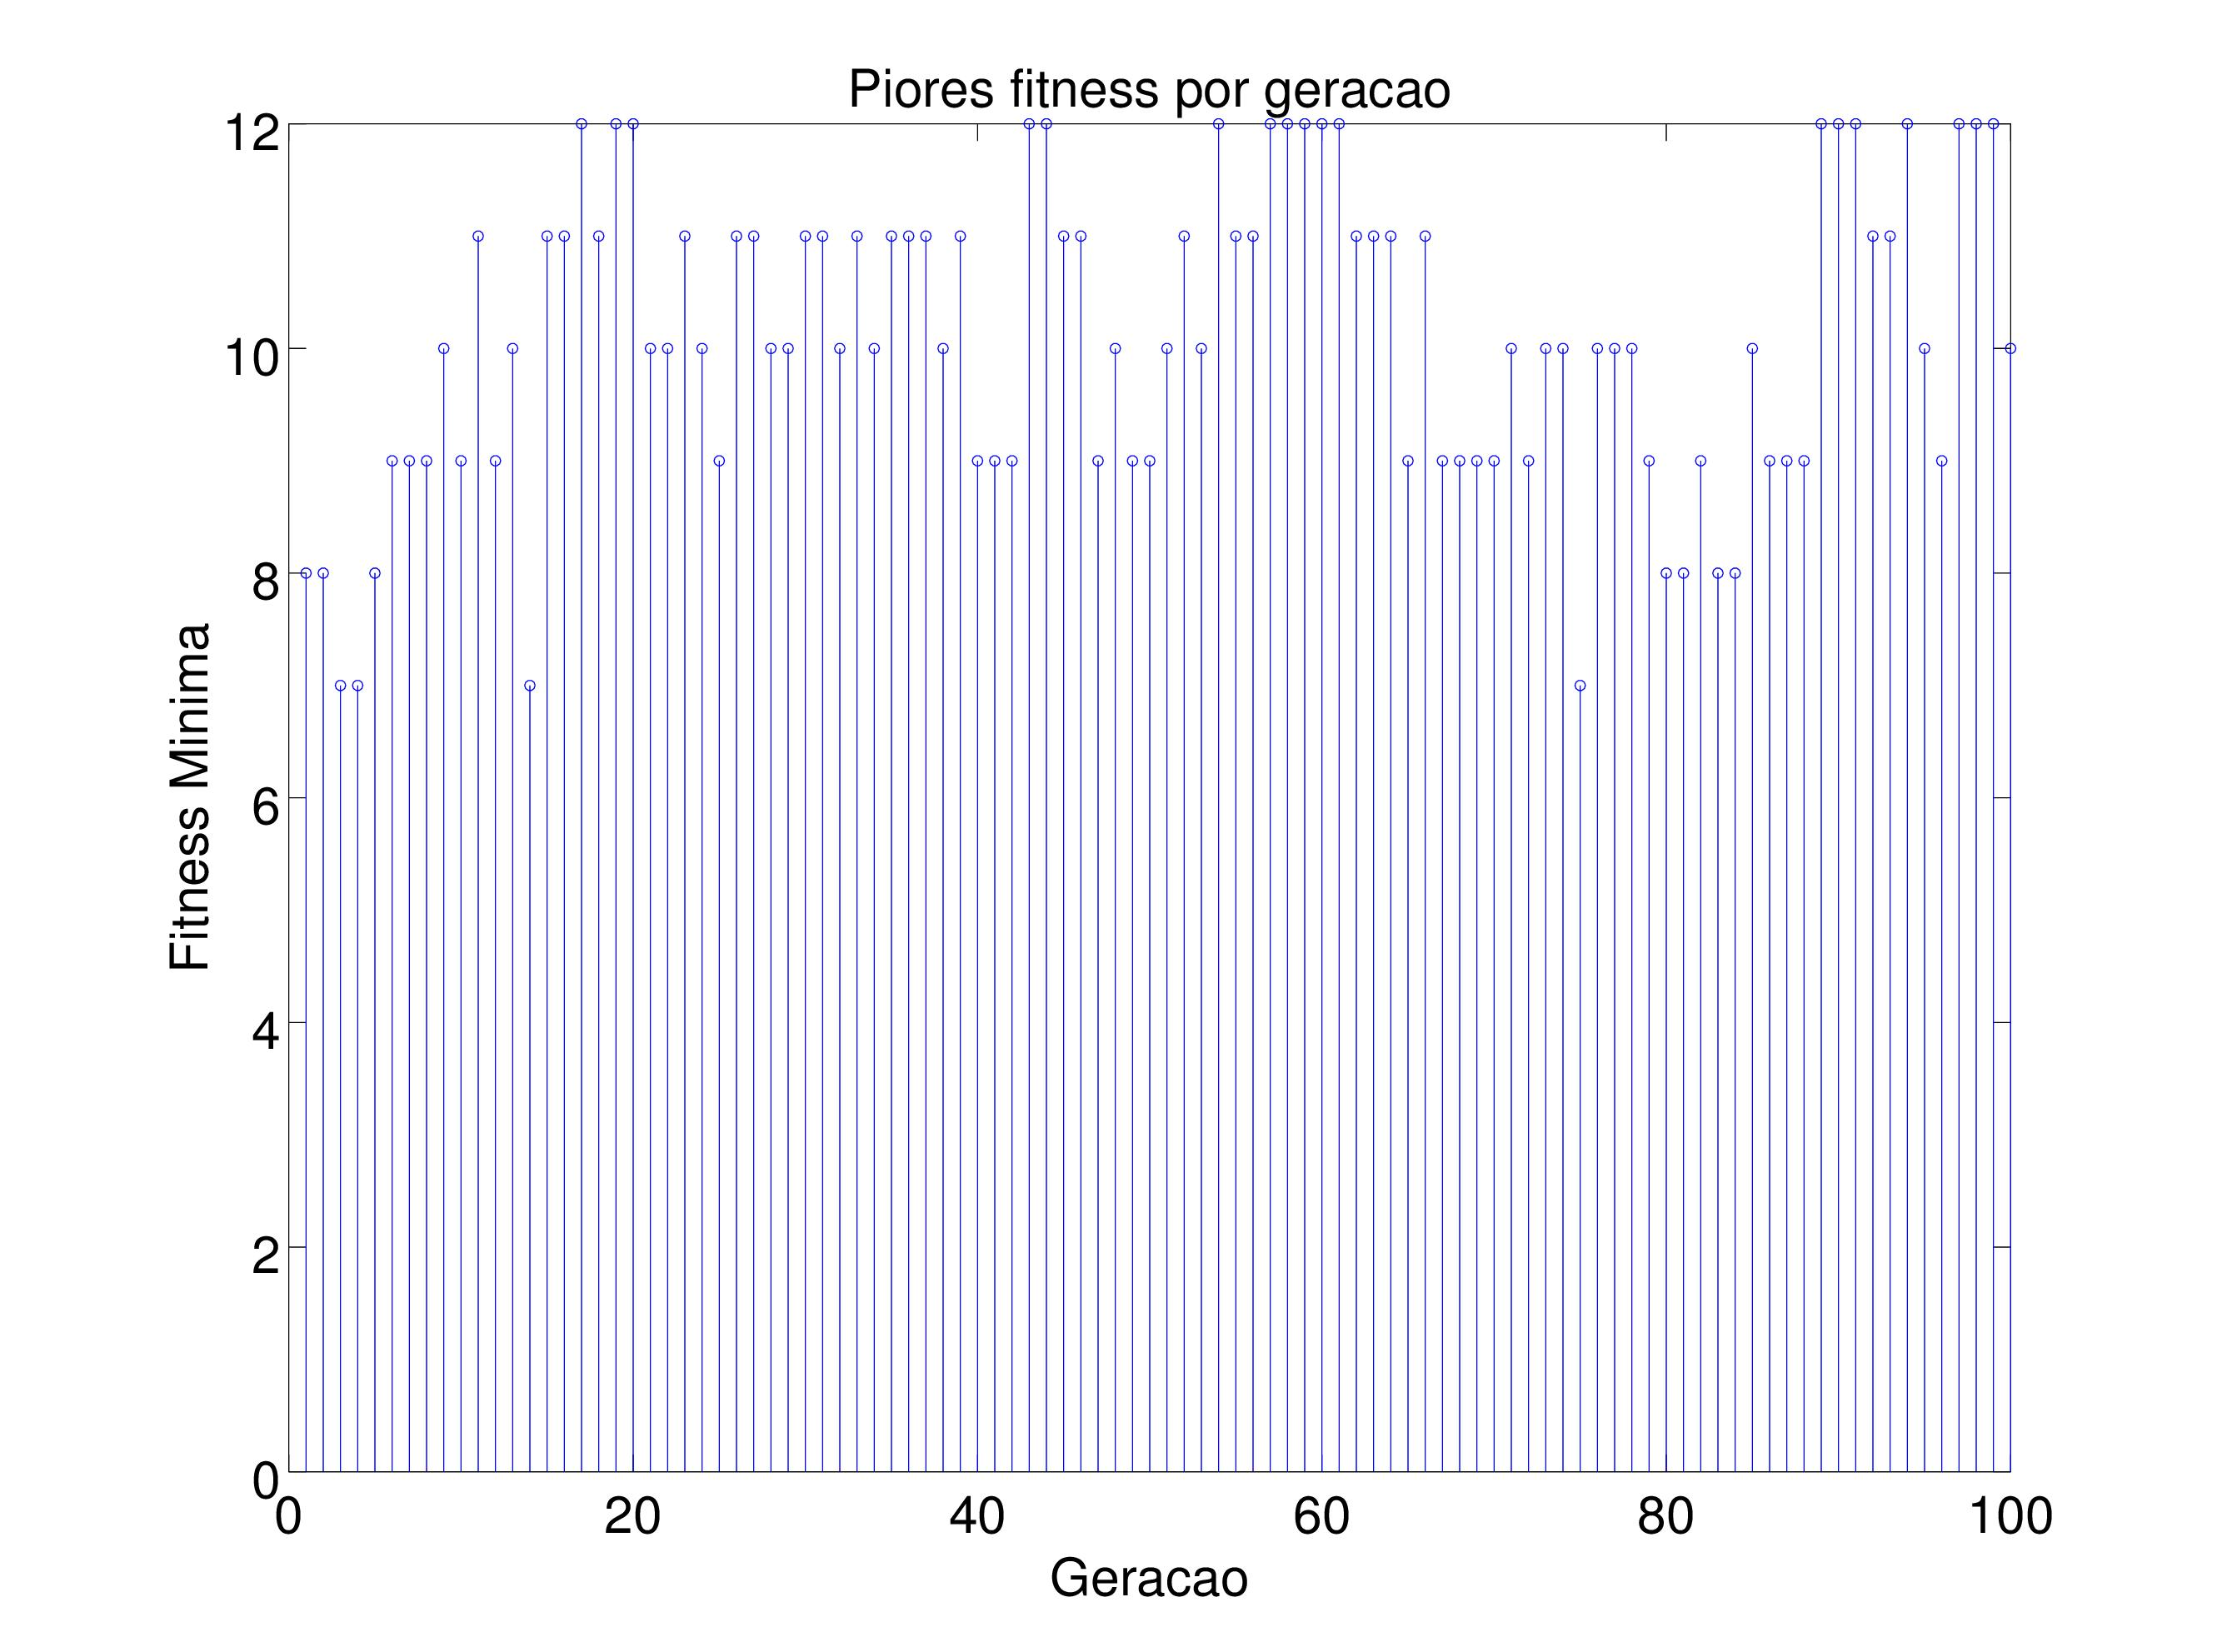
\includegraphics[width = 0.9\textwidth]{Q02_piores_fitness_100.jpg}
		\caption{Piores fitness encontradas ao longo de 100 gerações}
		\label{piores_fitness_100_q02}
	\end{figure}
	
	\begin{figure}[H]
		\centering
		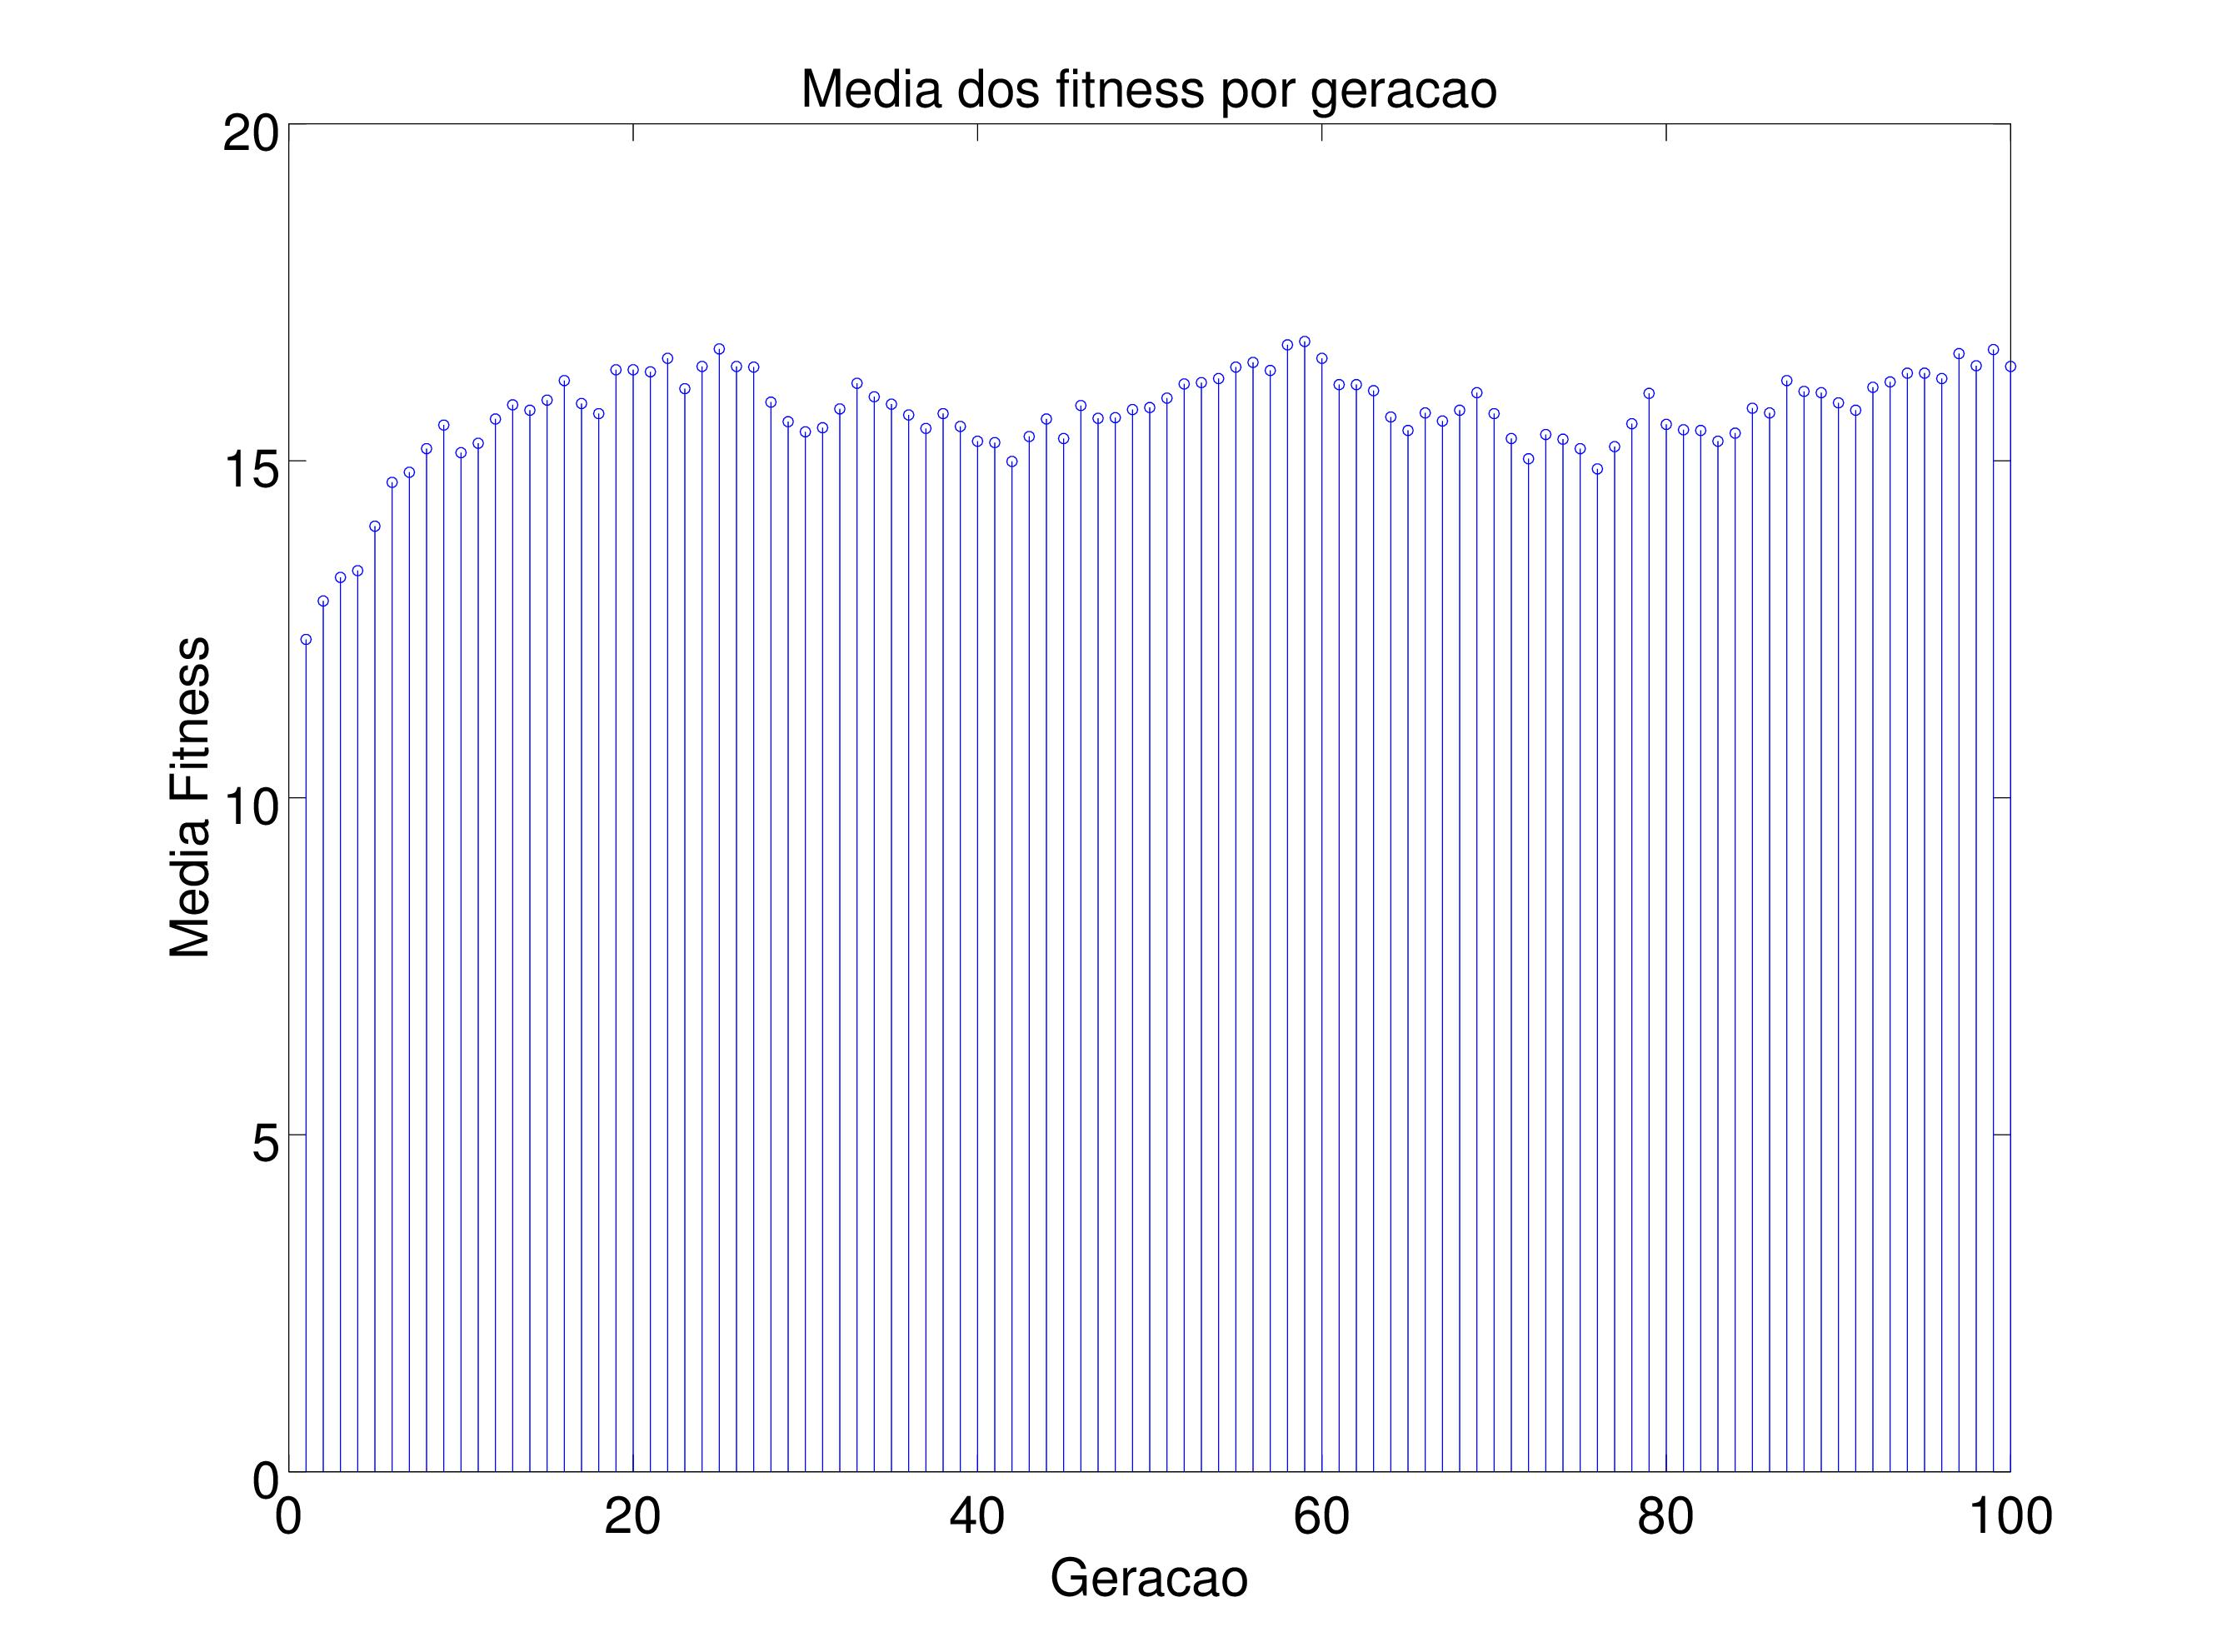
\includegraphics[width = 0.9\textwidth]{Q02_media_fitness_100.jpg}
		\caption{Média das fitness encontradas ao longo de 100 gerações}
		\label{media_fitness_100_q02}
	\end{figure}
	
	\paragraph{} De fato, as Figuras \ref{melhores_fitness_300_q02}, \ref{piores_fitness_300_q02} e \ref{media_fitness_300_q02} ilustram o comportamento da população quando 300 gerações são consideradas, em uma das execuções do algoritmo. É possível observar que existem indivíduos que se aproximam cada vez mais do ótimo global, em relação aos indivíduos das 100 primeiras gerações. Como todas as execuções atenderam ao critério de parada de número máximo de gerações avaliadas, não alcançando, portanto, o máximo global, a média das gerações é de 100 (para 100 gerações), e o desvio-padrão, 0.\\ 
	
	\begin{figure}[H]
		\centering
		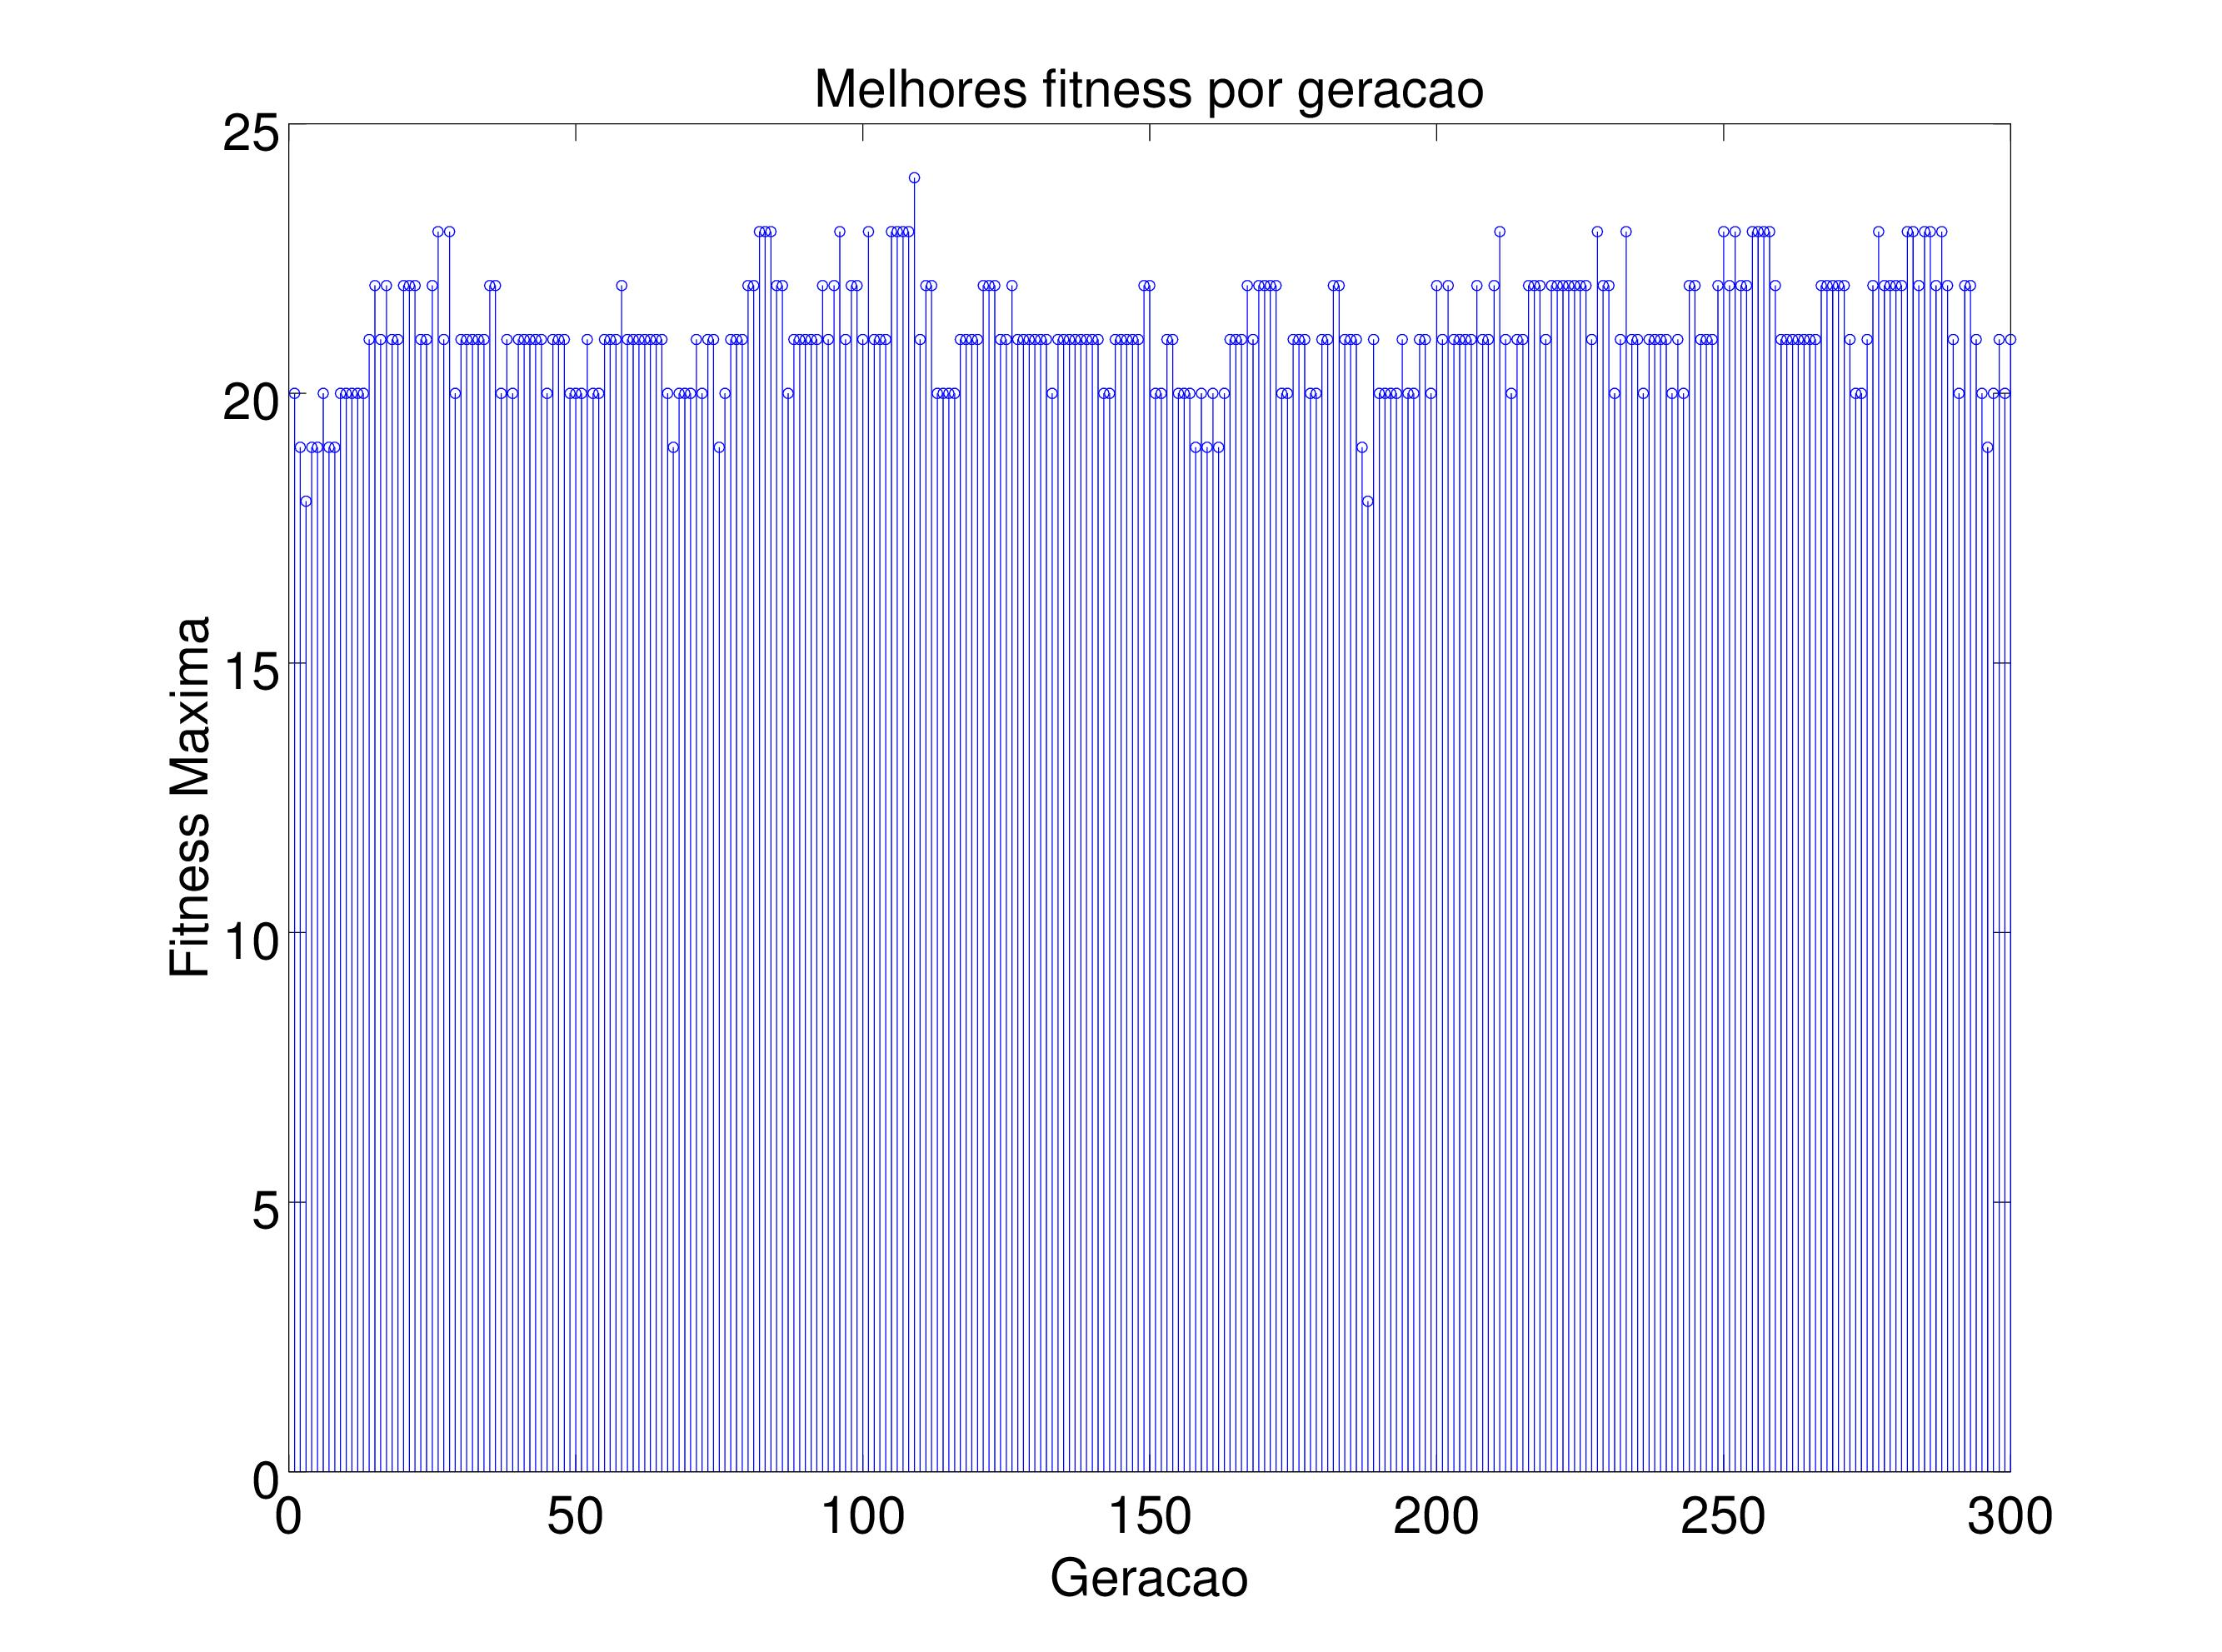
\includegraphics[width = 0.9\textwidth]{Q02_melhores_fitness_300.jpg}
		\caption{Melhores fitness encontradas ao longo de 300 gerações}
		\label{melhores_fitness_300_q02}
	\end{figure}
	
	\begin{figure}[H]
		\centering
		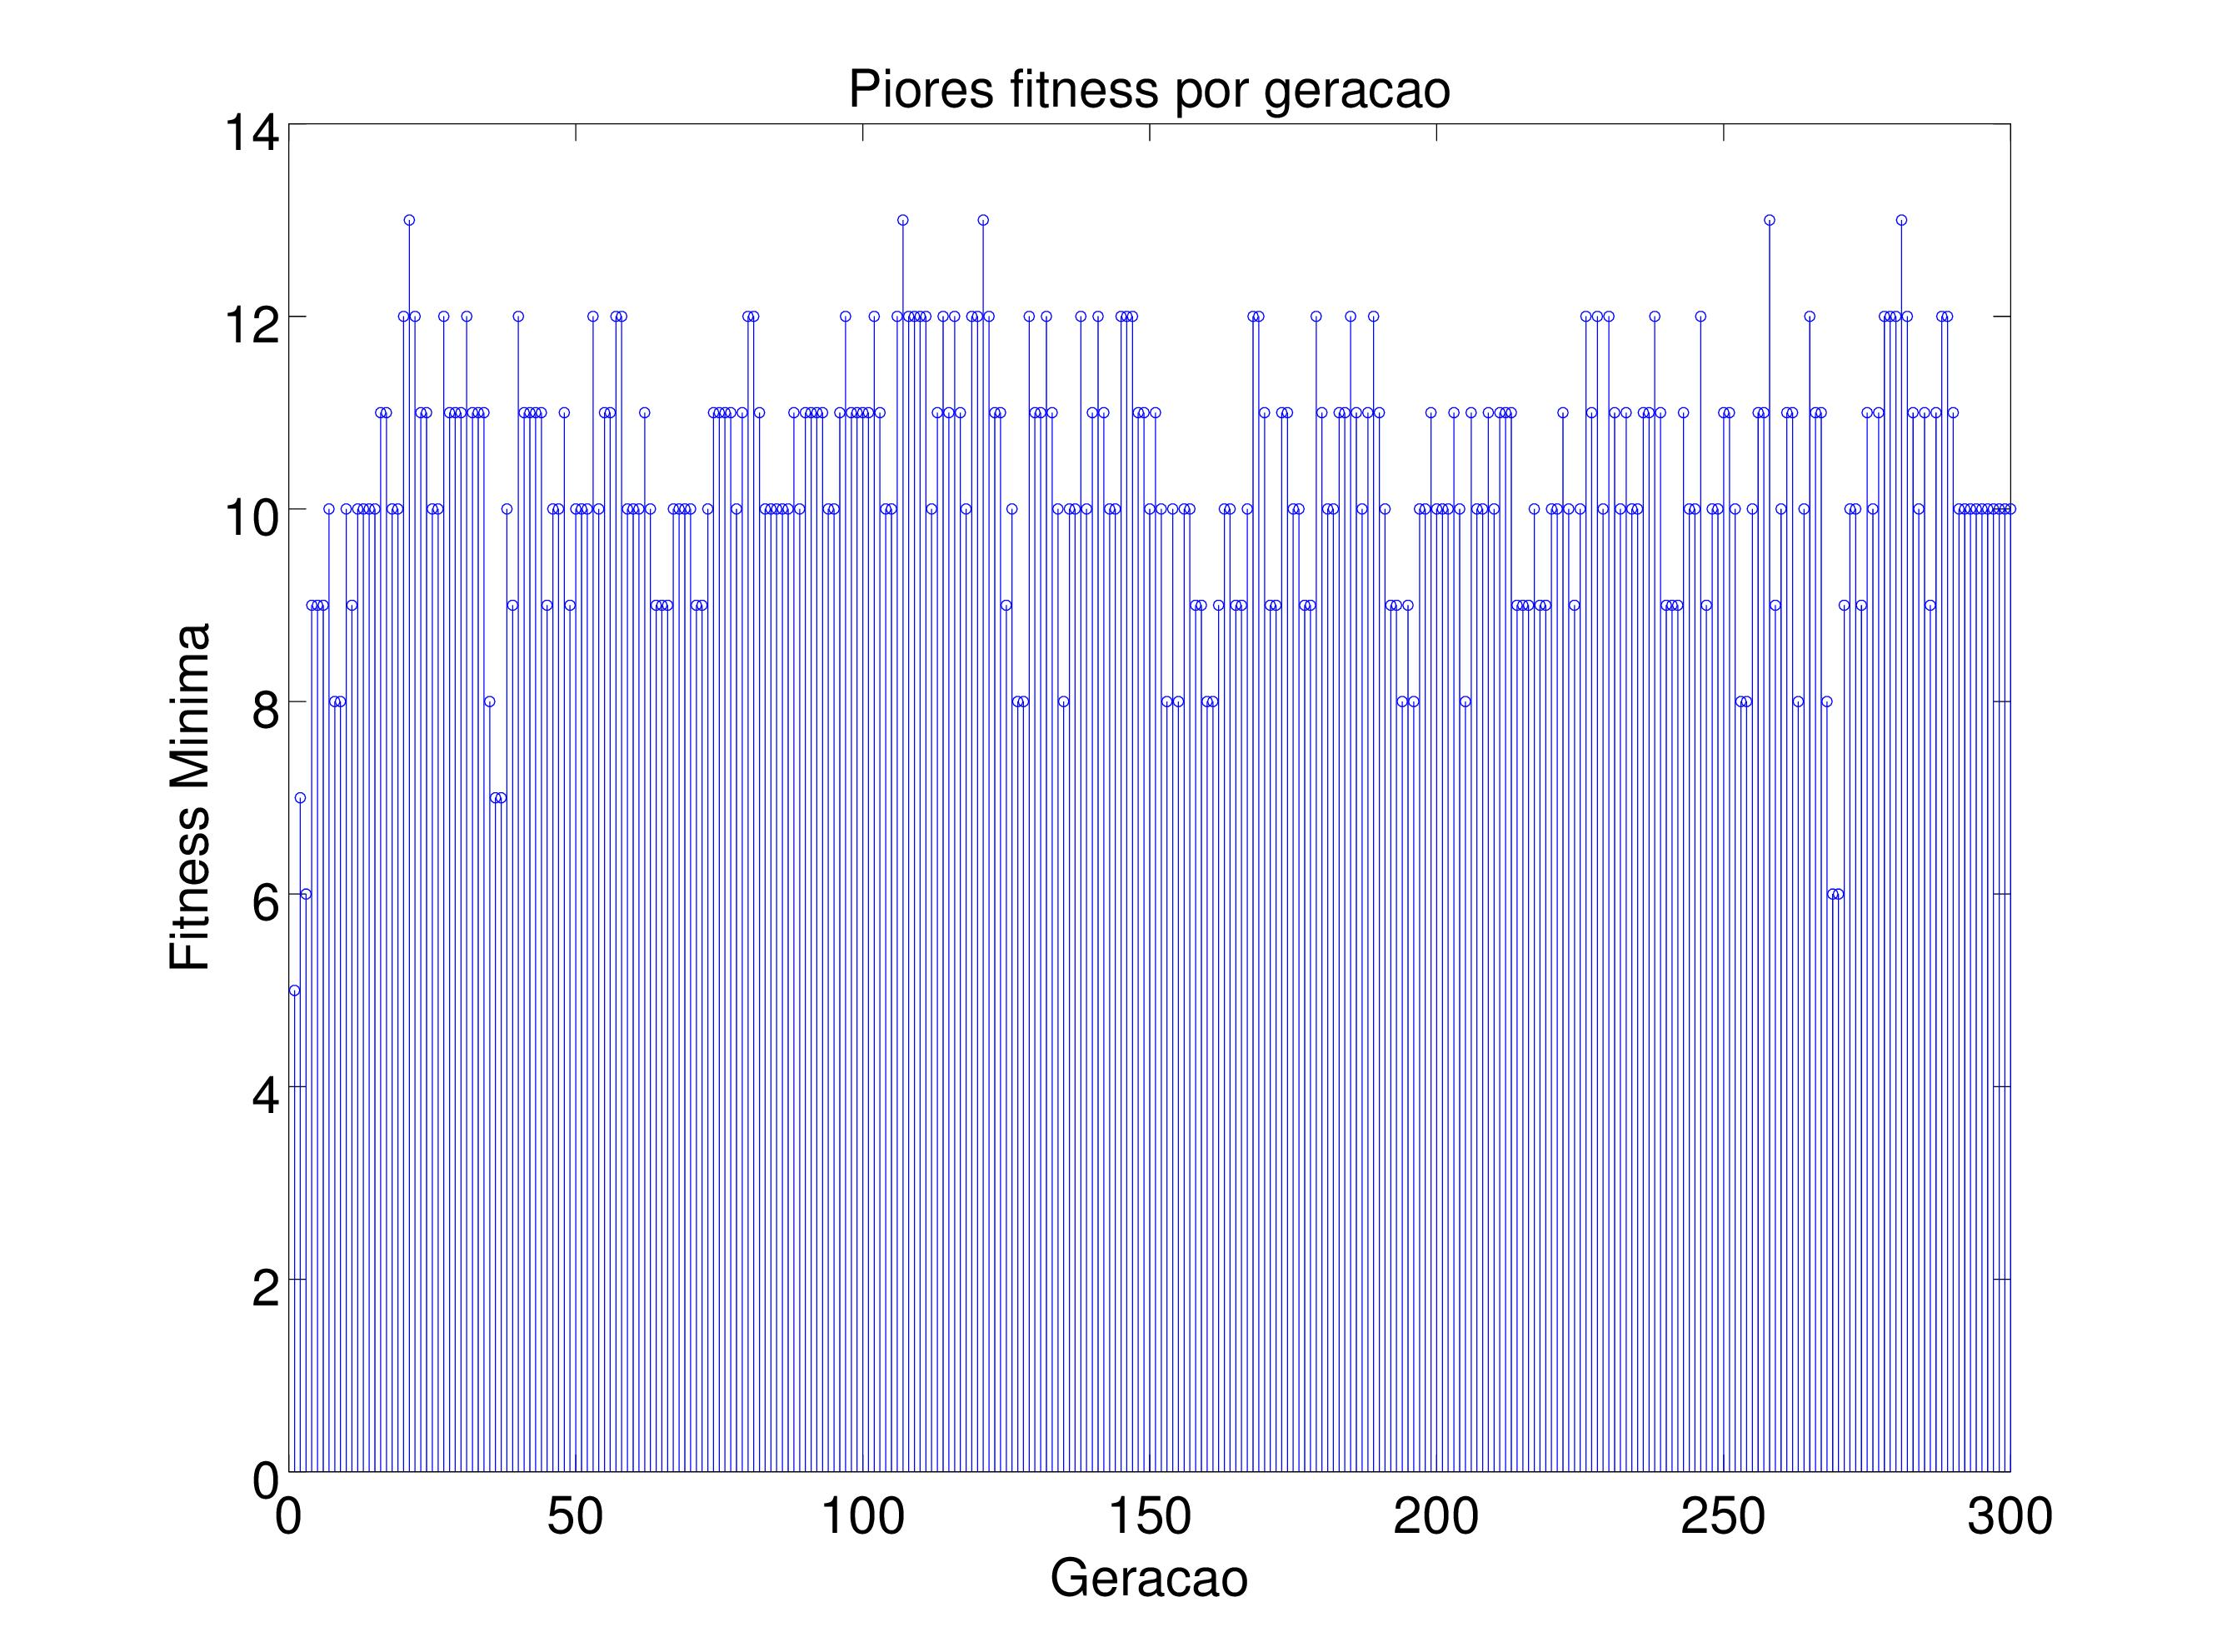
\includegraphics[width = 0.9\textwidth]{Q02_piores_fitness_300.jpg}
		\caption{Piores fitness encontradas ao longo de 300 gerações}
		\label{piores_fitness_300_q02}
	\end{figure}
	
	\begin{figure}[H]
		\centering
		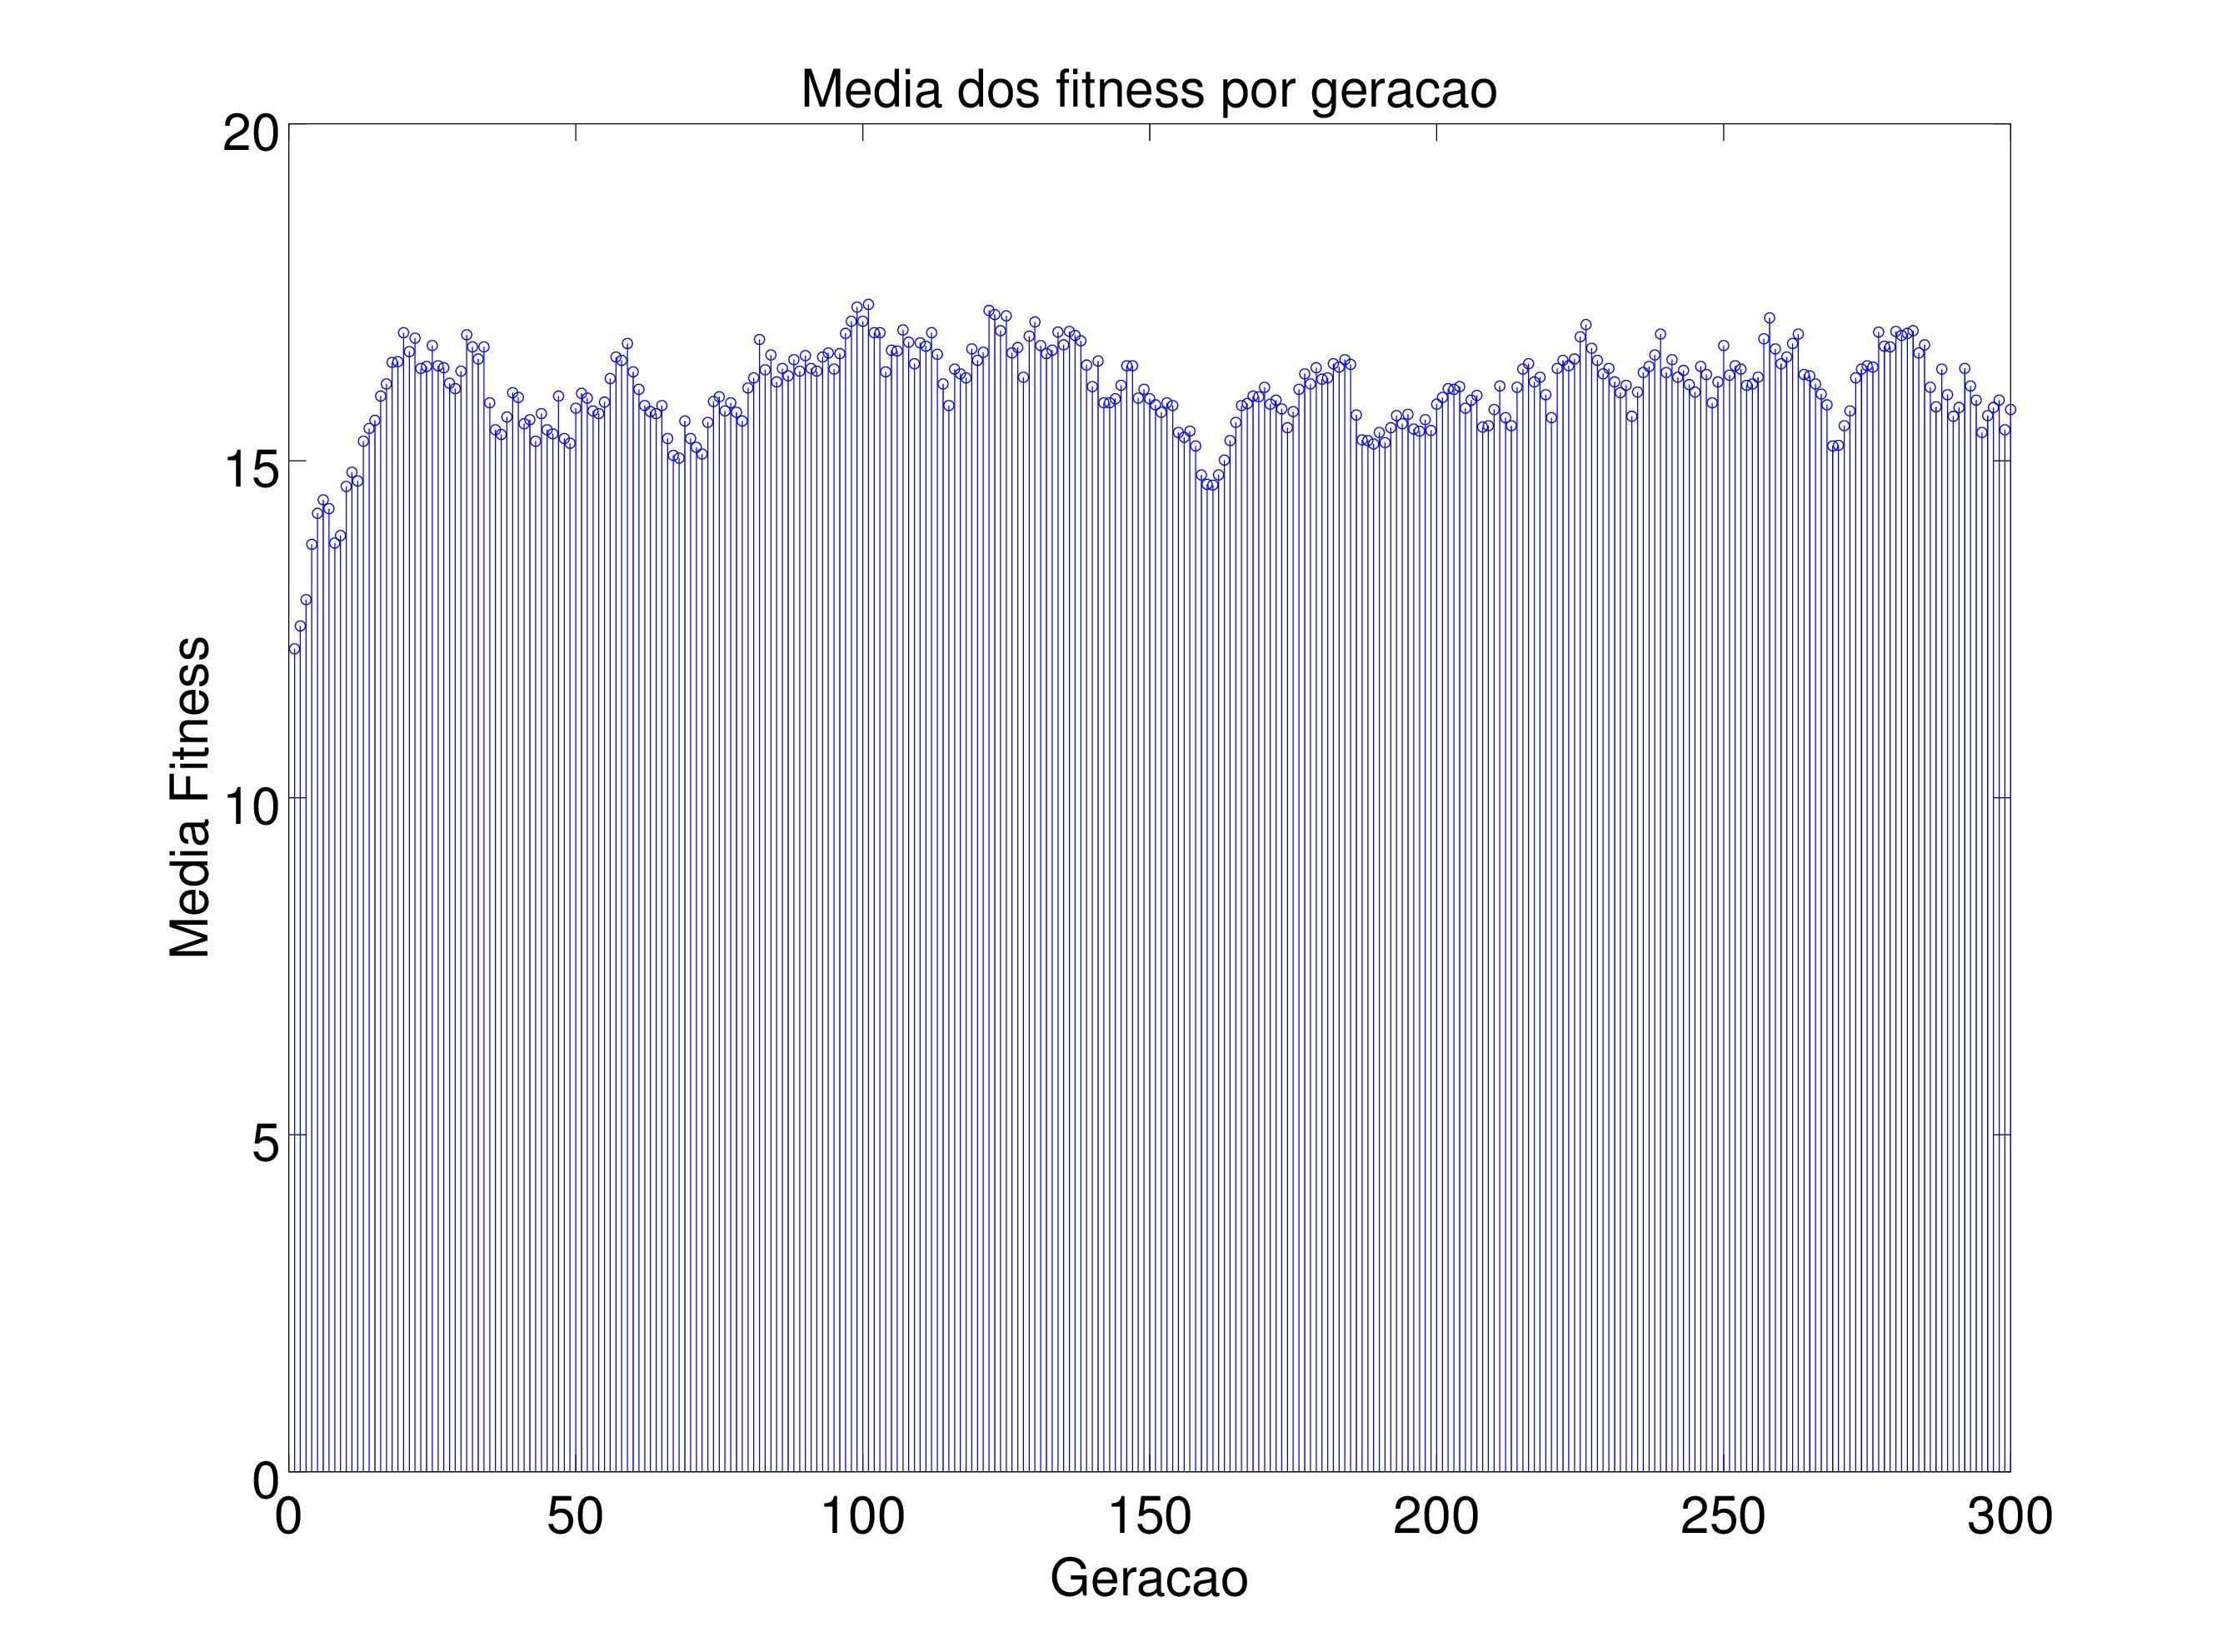
\includegraphics[width = 0.9\textwidth]{Q02_media_fitness_300.jpg}
		\caption{Média das fitness encontradas ao longo de 300 gerações}
		\label{media_fitness_300_q02}
	\end{figure}
	
	\section*{Questão 3}
	
	\textbf{\textit{3. Capítulo 4, Exercício 5:}}\\\\
	
	\textbf{Create an Evolutionary Strategy for the Ackley function with $n = 30$, using the set-up in Sect. 4.9.1 and a comma selection strategy. Make 100 independent runs, store the best value of each run and calculate the mean and standard deviation of these values.}
	
	\paragraph{} O código, feito em Octave, é apresentado abaixo:\\
	
	\begin{lstlisting}
clear all
close all
clc

N_pop = 30; % Tamanho da população
n = 30; % Quantidade de dimensões da função de Ackley
N_exec = 5; % Quantidade de execuções independentes do algoritmo
N_filhos = 200; % Número de filhos criados por geração
N_avaliacoes = 30000; % Quantidade de vezes que a função de Ackley será avaliada
N_ger = ceil(N_avaliacoes / N_pop); % Quantidade de gerações
tau = 1/sqrt(n);
tau_linha = 1/sqrt(2*sqrt(n));
epsilon = 0.1; % Valor mínimo para o passo de mutação
min_valores = Inf(N_exec, 2);
%melhores_solucoes = zeros(2*n, N_avaliacoes, N_exec);

for t = 1:N_exec

    P = [unifrnd(-30,30,n,N_pop); epsilon*ones(n,N_pop)]; % Inicialização aleatória da população
    ger = 1; % Geração atual
    opt = Inf;
    fitness = Inf(N_ger,N_pop);
    melhores_fitness = Inf(1, N_ger);
    media_fitness = zeros(1, N_ger);
    piores_fitness = Inf(1, N_ger);

    while (ger <= N_ger) && (min(fitness(ger,:)) ~= 0)
            
            % Cálculo dos fitness
            fitness(ger,:) = -20 * exp(-0.2 * sqrt((1/n) * sum(P(1:n,:).^2, 1))) - exp((1/n) * sum(cos(2 * pi * P(1:n,:)), 1)) + 20 + exp(1);
            opt = find(fitness(ger,:) == min(fitness(ger,:)), 1);
            melhores_fitness(ger) = min(fitness(ger,:));
            media_fitness(ger) = mean(fitness(ger,:)); 
            piores_fitness(ger) = max(fitness(ger,:));

            if min_valores(t,1) > min(fitness(ger,:))
                min_valores(t,:) = [min(fitness(ger,:)) ger];
            end

            % Mutação

            P_filhos = zeros(size(P,1), N_filhos); % 'N_pop' filhos de mutação e '(N_filhos - N_pop)' de recombinação
            
                % Mutação dos passos
            mutacoes = exp(tau * randn(n,N_pop)) .* (ones(n,1) * exp(tau_linha * randn(1,n))); % Alteração dos passos de mutação
            if ~isempty(find((mutacoes < epsilon), 1)) % Se houver algum passo menor que o mínimo
                mutacoes(mutacoes < epsilon) = epsilon; % Ajusta o passo para o mínimo aceitável
            end
                
            P_filhos((n+1):end, 1:N_pop) = mutacoes;

            % Mutação das soluções
                
            P_filhos(1:n, 1:N_pop) = P(1:n, 1:N_pop) + mutacoes .* randn(n,N_pop);

            % Recombinações

            for n_rec = 1:(N_filhos - N_pop)
                
                % Seleção dos pais                

                n_p1 = unidrnd(N_pop);
                n_p2 = unidrnd(N_pop);
                while (n_p2 == n_p1)
                    n_p2 = unidrnd(N_pop);
                end
                        
                sol_filho = zeros(n, 1);
                mut_filho = zeros(n, 1);
                sol_pai1 = P(1:n, n_p1);
                sol_pai2 = P(1:n, n_p2);
                mut_pai1 = P((n+1):end, n_p1);
                mut_pai2 = P((n+1):end, n_p2);

                % Recombinação discreta (soluções)
                
                z = unifrnd(0,1, n, 1);

                for i = 1:length(z)
                    if z(i) < 0.5
                        sol_filho(i) = sol_pai1(i);
                    else
                        sol_filho(i) = sol_pai2(i);
                    end
                end

                % Recombinação intermediária (passos)

                mut_filho = (mut_pai1 + mut_pai2)/2;

                P_filhos(:, (N_pop+n_rec)) = [sol_filho; mut_filho];
                    
            end

            % Seleção dos sobreviventes

            % Generacional com 'N_pop' filhos mais aptos

            fitness_filhos = ones(1,size(P_filhos,2));
            
            fitness_filhos = -20 * exp(-0.2 * sqrt((1/n) * sum(P_filhos(1:n,:).^2, 1))) - exp((1/n) * sum(cos(2 * pi * P_filhos(1:n,:)), 1)) + 20 + exp(1);

            idx = zeros(1,N_pop);

            for i = 1:N_pop

                idx(i) = find(fitness_filhos == min(fitness_filhos), 1);
                fitness_filhos(idx(i)) = Inf;

            end

            P = P_filhos(:, idx);

            ger = ger + 1;

    end

    if (ger <= N_ger)
        fitness = fitness(1:ger, :);
    end

end


	\end{lstlisting}
	
	\paragraph{}	 Abaixo, estão definidos alguns dos elementos essenciais de Algoritmos Evolucionários (os quais estão definidos na Seção 4.9.1, citada no enunciado do problema).\\
	
	\begin{itemize}
		
		\item[\textbf{1.}] \textbf{Representação}
		
		\paragraph{} A representação consiste em um vetor de números reais. Esse vetor contém 60 elementos: os 30 primeiros, correspondem à solução propriamente dita, ao passo que os 30 últimos representam os passos que serão usados na mutação (e que, também, estão sujeitos à mutação). Nessa questão, adotou-se que cada gene apresenta um passo distinto. O fitness de cada indivíduo é definido como sendo o resultado da função de Ackley, aplicado aos 30 primeiros genes.\\
		
		\item[\textbf{2.}] \textbf{Seleção de pais}
	
		\paragraph{} Todos os indivíduos da população são possíveis pais, que serão usados na recombinação. A seleção, nesse caso, é puramente aleatória, ou seja, sorteiam-se dois pais da população total para realizar a recombinação.\\
		
		\item[\textbf{3.}] \textbf{Mutação}
		
		\paragraph{} Cada indivíduo sofre mutação e o indivíduo resultante passa a integrar a população de filhos (portanto, ele não substitui o indivíduo que o gerou). Antes da mutação dos genes referentes à solução, os passos sofrem mutações, segundo a seguinte fórmula:\\
		
		\begin{equation*}
		\sigma_i^{'} = \sigma_i \times e^{\tau^{'} \times N(1,0) + \tau \times N_i(0,1)}
		\end{equation*}
		
		\paragraph{} Na equação acima, $\sigma_i$ é o passo pré-mutação associado ao gene $i$	; $\tau^{'}$ e $\tau$ são constantes definidas, respectivamente, como $\frac{1}{\sqrt{2n}}$ e $\frac{1}{\sqrt{2 \sqrt{n}}}$, com $n = 30$; $N(1,0)$ é uma amostra de uma distribuição Gaussiana, com média 0 e desvio-padrão 1; e $N_i(0,1)$ é o $i$-ésimo sorteio dessa distribuição, cujo valor entra no cálculo do passo associado ao gene $i$. Adotou-se, também, um valor mínimo para o passo, de modo a evitar que passos muito pequenos fossem considerados (o que significaria em uma mudança muito pouco impactante no gene). Para essa questão, esse valor mínimo foi fixado em 0.1.\\
		
		\paragraph{} Após a mutação dos passos, cada gene associado à solução sofre mutação da seguinte forma: $x_i^{'} = x_i + \sigma_i^{'} \times N_i(0,1)$.	
	
		\item[\textbf{4.}] \textbf{Recombinação}
		
		\paragraph{} Com os pais selecionados, duas estratégias de recombinação são usadas. Para as regiões dos genótipos que contêm as soluções, a recombinação é dita \emph{discreta}. Nesse caso, um número da distribuição uniforme entre 0 e 1 é sorteado e seu valor é comparado a um limiar, usualmente 0.5. Caso ele seja maior do que o limiar, o filho gerado recebe o gene de um dos pais; caso contrário, recebe do outro. Já para as regiões referentes ao passo, a recombinação é dita \emph{intermediária}, isto é, cada novo passo é dado pela média aritmética dos passos correspondentes dos pais em questão. Vale ressaltar que a recombinação, nesse caso, resulta em somente 1 filho.\\
		
		\item[\textbf{5.}] \textbf{Seleção de sobreviventes}
		
		\paragraph{} A seleção de sobreviventes é denominada ($\mu$,$\lambda$) e corresponde à uma seleção generacional. No entanto, como a quantidade de filhos é superior à população original (nesse caso, 200 filhos são gerados, enquanto que a população tem tamanho 30), é feita uma seleção dos melhores filhos, os quais integrarão a nova geração. Para isso, os filhos são ranqueados segundo o valor de seu fitness (função de Ackley), sendo selecionados, portanto, os 30 mais aptos.\\
		
		\item[\textbf{7.}] \textbf{Inicialização}
		
		\paragraph{} A inicialização é feita de forma aleatória, com a região de genes referentes à solução sendo inicializados com valores entre -30 e 30, enquanto que a região dos passos é inicializada de forma igual, para todos os passos e indivíduos, com cada passo igual ao mínimo aceitável (no caso, definiu-se que esse mínimo seria de 0.1).\\		
		
		\item[\textbf{7.}] \textbf{Condição de parada}
		
		\paragraph{} Na Seção 4.9.1 do livro, é sugerido que a condição de parada seja após se avaliarem 200000 vezes a função de Ackley, ou até que o mínimo global seja alcançado. Entretanto, devido ao elevado tempo de execução, reduziu-se essa condição: a função de Ackley será avaliada 30000 vezes, em vez de 200000. Além disso, como em cada geração sempre são feitas 30 análises dessa função (1 para cada indivíduo), reescreveu-se essa condição de parada em função do número de gerações que seriam necessárias para se alcançar essa quantidade de avaliações. Portanto, a condição de parada passou a ser até que 1000 gerações fossem consideradas, ou que o mínimo global fosse encontrado.\\
	\end{itemize}
	
	\paragraph{} Para essa questão, em nenhuma das vezes que se executou o algoritmo, o mínimo global foi alcançado. A Figura \ref{melhores_fitness_5_exec_q03} mostra as melhores fitness encontradas em 5 rodadas distintas do algoritmo. Analisando algumas rodadas do algoritmo, notou-se que ele ficou preso durante um certo número de gerações em um mínimo local, conforme se nota na Figura \ref{media_fitness_q03}, a qual mostra a fitness média dos indivíduos em cada geração. Eventualmente, por meio de mutação e recombinação, novos indivíduos mais aptos são gerados, e o algoritmo consegue escapar do mínimo local. O comportamento observado sugere que após um número suficientemente alto de gerações, o mínimo global será alcançado.\\
	
	\begin{figure}[H]
		\centering
		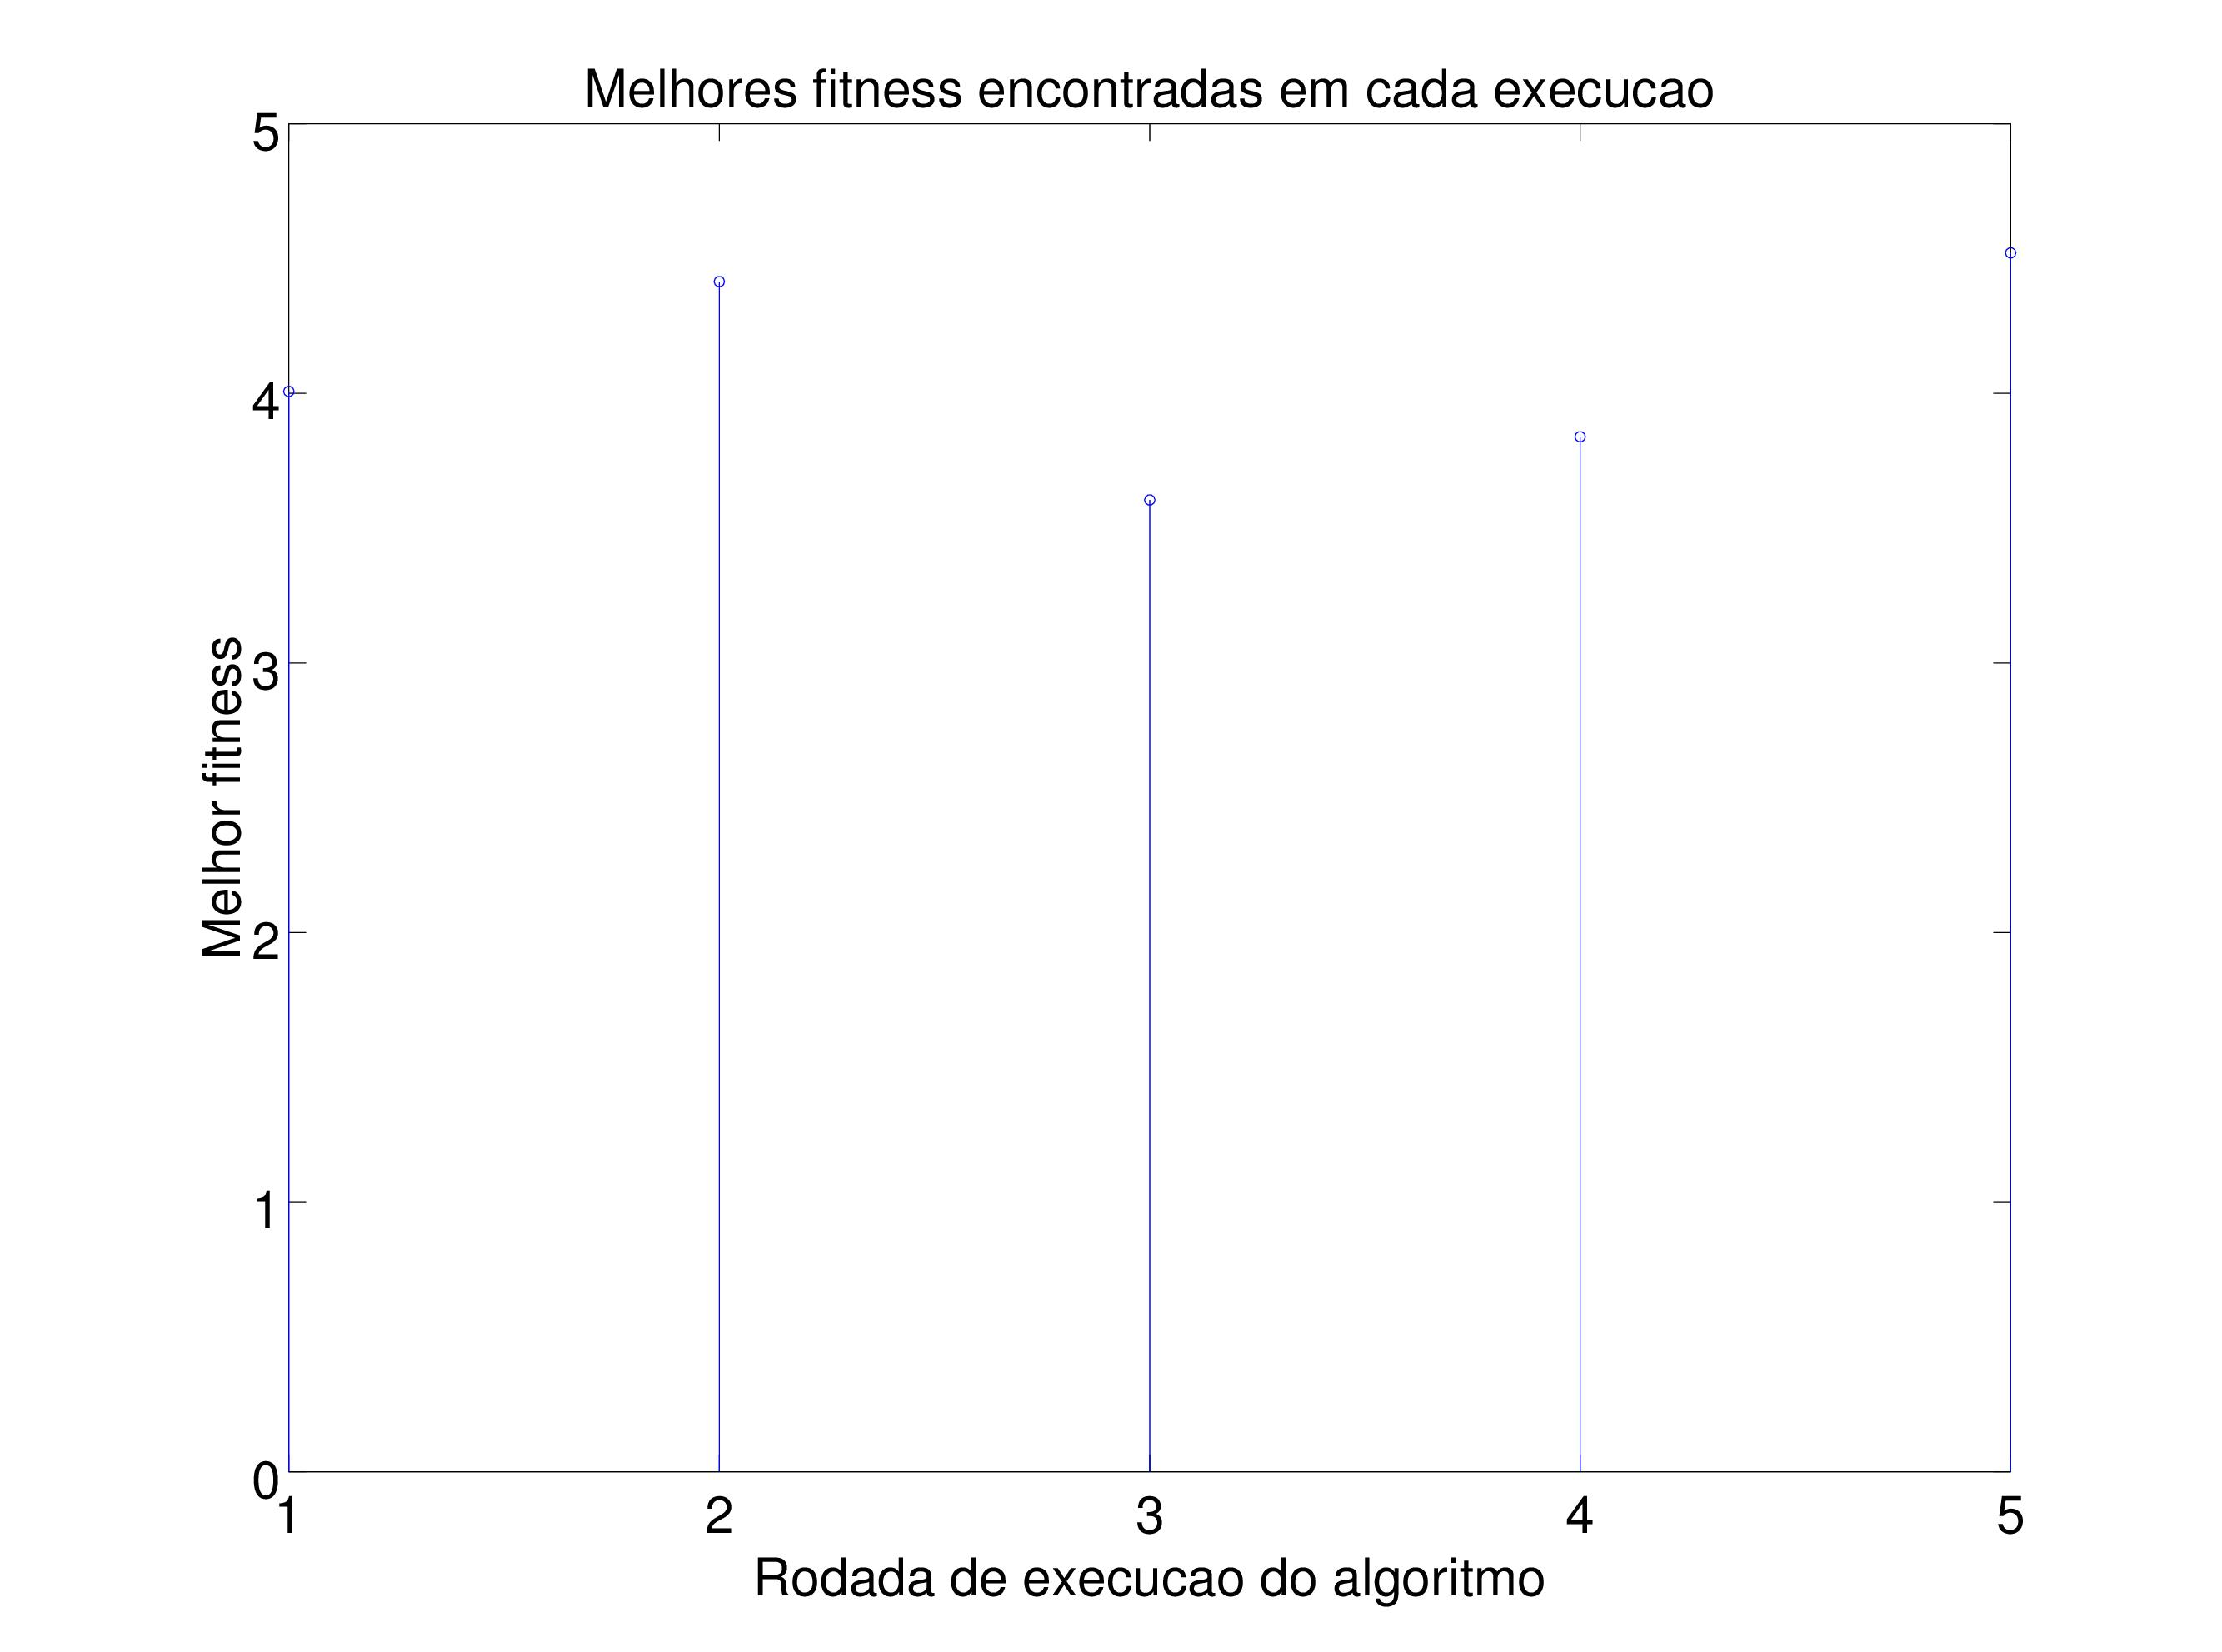
\includegraphics[width = 0.9\textwidth]{Q03_melhores_fitness.jpg}
		\caption{Melhores fitness encontradas em execuções independentes do algoritmo}
		\label{melhores_fitness_5_exec_q03}
	\end{figure}
	
	\begin{figure}[H]
		\centering
		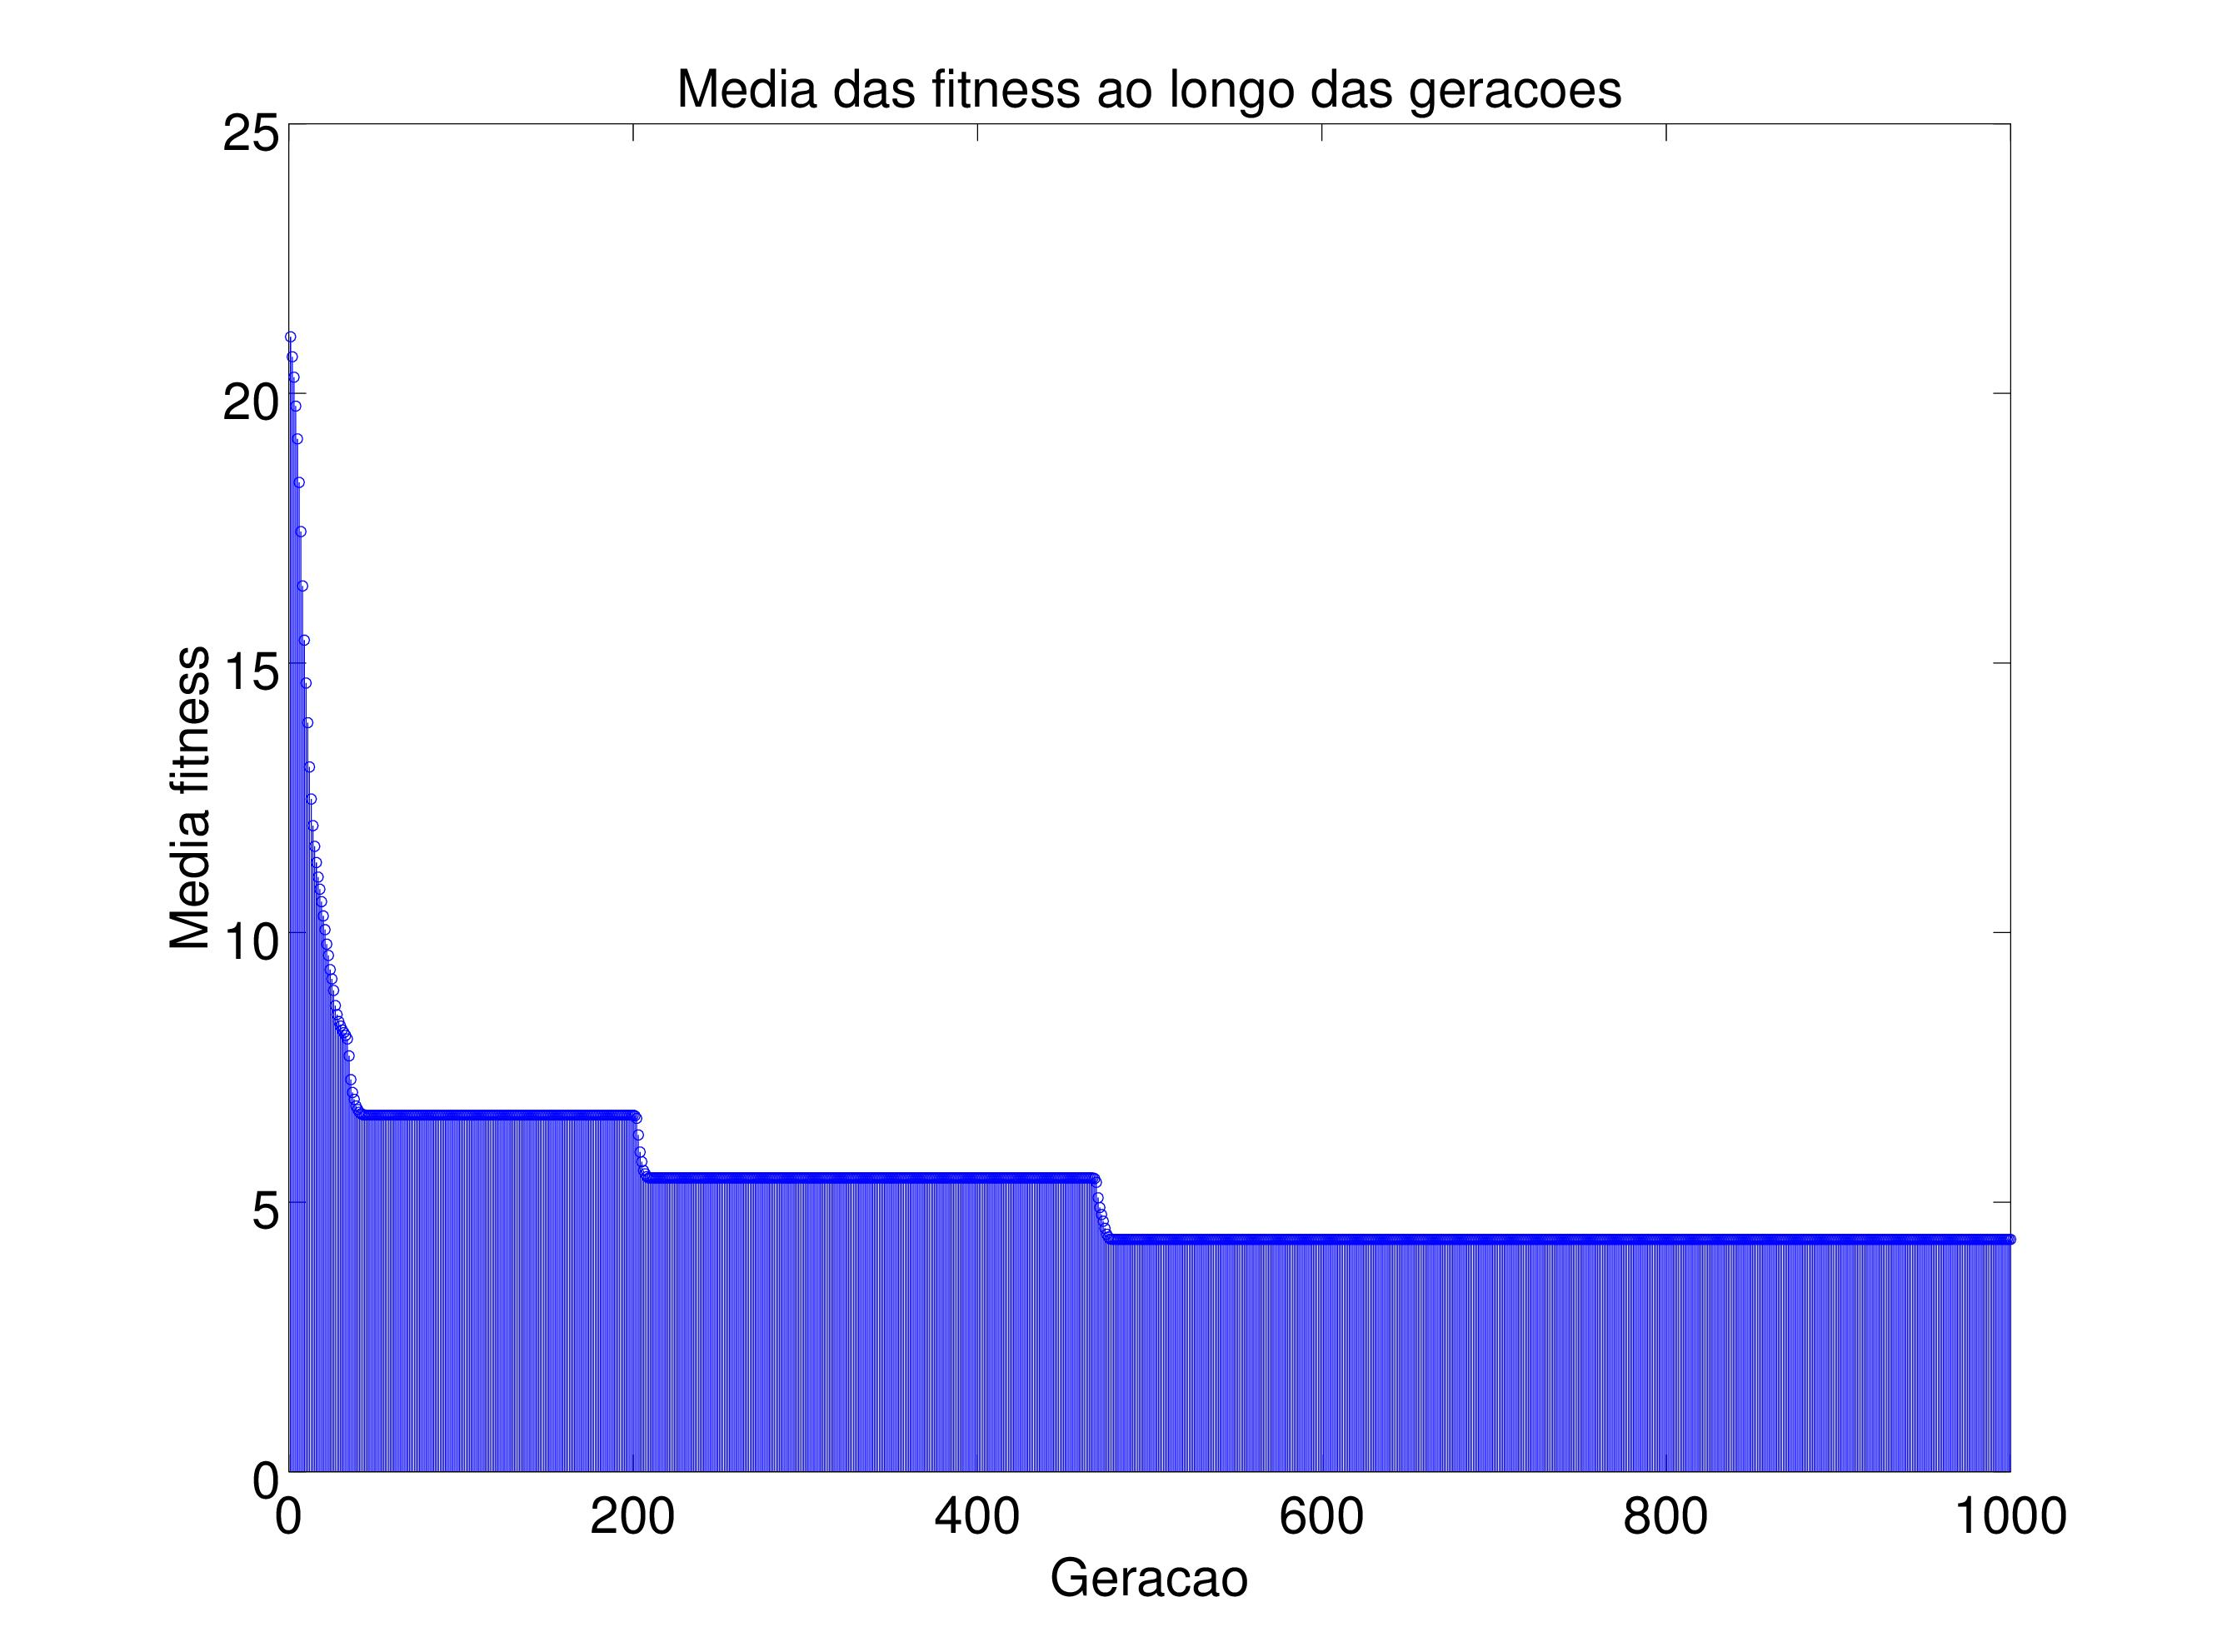
\includegraphics[width = 0.9\textwidth]{Q03_media_fitness.jpg}
		\caption{Média das fitness encontradas em cada geração, em uma execução do algoritmo}
		\label{media_fitness_q03}
	
	\end{figure}
	
	\section*{Questão 4 (Bônus)}
	
	\textbf{4. Implemente um algoritmo genético simples (SAG), de modo a solucionar o problema das 8 rainhas.}\\

	\paragraph{} Nessa questão bônus, optou-se por resolver o problema clássico das 8 rainhas, utilizando Algoritmos Evolucionários (mais especificamente, Algoritmos Genéticos). Os elementos do algoritmo são definidos a seguir:\\
	
	\begin{itemize}
		\item[\textbf{1.}] \textbf{Representação}
		
		\paragraph{} A representação escolhida consiste em um genótipo, formado por um vetor de inteiros de 8 elementos, com valores possíveis entre 1 e 8, o qual codifica um fenótipo referente a uma matriz 8x8, correspondente a um tabuleiro de xadrez. Essa matriz é composta por colunas que apresentam elementos iguais a 0, exceto em uma única linha, na qual o elemento em questão vale 1. Cada coluna contém uma linha diferente que abriga esse valor 1. Os números que compõem o genótipo explicitam, exatamente, para cada coluna, a linha que contém o elemento 1. Além disso, colunas distintas não podem ter a mesma linha com elemento 1 (ou seja, não há elementos repetidos no genótipo de cada indivíduo). Os valores 1 representam a posição das rainhas no tabuleiro. Considere, por exemplo, o genótipo representado por $G = [1 \quad 4 \quad 5 \quad 3 \quad 8 \quad 6 \quad 7 \quad 2]$. O fenótipo associado a esse genótipo é exibido a seguir:\\
		
		\begin{equation*}
		\begin{array}{cccccccc}
		1 & 0 & 0 & 0 & 0 & 0 & 0 & 0 \\ 
		0 & 0 & 0 & 0 & 0 & 0 & 0 & 1 \\ 
		0 & 0 & 0 & 1 & 0 & 0 & 0 & 0 \\ 
		0 & 1 & 0 & 0 & 0 & 0 & 0 & 0 \\ 
		0 & 0 & 1 & 0 & 0 & 0 & 0 & 0 \\ 
		0 & 0 & 0 & 0 & 0 & 1 & 0 & 0 \\ 
		0 & 0 & 0 & 0 & 0 & 0 & 1 & 0 \\ 
		0 & 0 & 0 & 0 & 1 & 0 & 0 & 0
		\end{array} 
		\end{equation*}
		
		\paragraph{} O motivo de se escolher essa representação é que ela descarta soluções que contenham rainhas situadas na mesma linha ou coluna, as quais corresponderiam a violações das restrições do problema (sendo, portanto, soluções inválidas). Isso diminui o espaço de busca do algoritmo. A fitness é calculada através da contagem quantas rainhas, no tabuleiro, estão a salvo, isto é, que estão livres de quaisquer ataques. Para tal, não deve haver rainhas na mesma diagonal, linha ou coluna .\\
		
		\item[\textbf{2.}] \textbf{Seleção de Pais}
				
		\paragraph{} A seleção de pais é feita levando-se em conta a aptidão de cada indivíduo (proporcional ao fitness de cada um). O tamanho da população reprodutora é igual ao da população (no caso, 100) e a montagem da população reprodutora é feita aplicando-se o algoritmo ``Stochastic Universal Sampling". Cada par de pais gera um par de filhos.\\
		
		\item[\textbf{3.}] \textbf{Recombinação}
		
		\paragraph{} Com a população de reprodutores montada, começa-se a geração da população de filhos. Os pais são sorteados aleatoriamente na população reprodutora e, uma vez selecionados, podem ou não sofrer o processo de recombinação. Caso não sofram, os filhos gerados são, simplesmente, cópias de ambos os pais. Caso contrário, o processo de recombinação adotado é conhecido como \emph{``One-point Crossover"} e consiste, basicamente, em sortear uma posição aleatória do genótipo, dividindo-o em duas regiões. A montagem dos filhos é feita, então, combinando metades distintas de cada pai (filho 1 = metade 1 do pai 1 + metade 2 do pai 2 e filho 2 = metade 1 do pai 2 + metade 2 do pai 1). Entretanto, vale ressaltar que, para a representação escolhida, não deve haver elementos repetidos no genótipo. Com isso, após se copiar a primeira metade de um pai para um filho, a segunda metade desse filho é montada, analisando cada gene do outro pai. Se um gene da segunda metade desse pai já existir na primeira metade do filho em questão, ele não é copiado e analisa-se o próximo gene desse pai. O gene só é copiado se não for repetido. Caso se chegue ao fim da segunda metade do pai e a segunda metade do filho não tenha sido finalizada, continua-se a análise do genótipo deste pai do começo, ou seja, de sua primeira metade, até se encontrar os genes que faltam ao filho e copiá-los.\\
		
		\item[\textbf{4.}] \textbf{Mutação}
		
		\paragraph{} Após gerados os filhos, podem ocorrer, ainda, mutações nos genes. Arbitrou-se que a mutação ocorre somente nos filhos gerados e que o novo indivíduo gerado pela mutação substitui sua versão pré-mutação (ao invés de se preservar os indivíduos pré- e pós-mutação). A mutação consiste em trocar a posição de dois elementos no genótipo (por exemplo, trocar a posição dos genes 2 e 5; o gene 5 passa a ocupar a posição 2, ao passo que o gene 2, a posição 5.).\\
		
		\item[\textbf{5.}] \textbf{Seleção de Sobreviventes}
		
		\paragraph{} A seleção dos sobreviventes é puramente generacional, ou seja, toda a população de filhos compõe a geração seguinte, enquanto que todos os pais são descartados.\\
		
		\item[\textbf{6.}] \textbf{Inicialização}
		
		\paragraph{} A inicialização da população é feita de forma aleatória (preservando a condição de que um genótipo não contém elementos repetidos). Para tal, inicializou-se o primeiro indivíduo com genótipo $G_1 = [1 \quad 2 \quad 3 \quad 4 \quad 5 \quad 6 \quad 7 \quad 8]$ e os indivíduos subsequentes são gerados, trocando a posição de dois genes do indivíduo anterior. Isso é repetido até que se gere o tamanho da população desejada.\\
		
		\item[\textbf{7.}] \textbf{Condição de Parada}
		
		\paragraph{} O algoritmo encerra sua execução após se atingir um determinado número de gerações ou uma solução ótima seja encontrada.\\
	\end{itemize}
	
	\paragraph{} O código, em Octave, que implementa a solução, é exposto a seguir. O algoritmo foi executado 1000 vezes, sendo a geração média, na qual a solução ótima apareceu, igual a 5.55 ($\approx 6$), com desvio-padrão de $\approx 5.02$. \\
	
	\begin{lstlisting}
clear all;
close all;
clc;

N_pop = 100; % Tamanho da população
N_ger = 20; % Quantidade de gerações
N_col = 8; % Número de colunas do tabuleiro
N_exec = 100; % Número de execuções independentes do algoritmo
p_rec = 0.8;
p_mut = 0.1;
ger_otimas = zeros(1,N_exec); % Armazena a geração em que a solução ótima ocorreu


for t = 1:N_exec

    fitness = zeros(N_ger,N_pop); % Número de rainhas salvas
    n = 1; % Geração atual
    max_fitness = 0;
    %% Inicialização aleatória dos genótipos

    P = zeros(N_pop, N_col);

    P(1,:) = 1:N_col;

    for i = 2:N_pop

        P(i,:) = P((i-1),:);

        r1 = unidrnd(N_col);
        r2 = unidrnd(N_col);
        while (r2 == r1)
            r2 = unidrnd(N_col);
        end
        
        aux = P(i,r1);
        P(i,r1) = P(i, r2);
        P(i,r2) = aux;
    end

    while (n <= N_ger) && (max_fitness ~= 8)

        %% Decodificação em fenótipo e cálculo de fitness

        F = zeros(N_col, N_col, N_pop);
        for i = 1:size(P,1);

            k = 1;
            for j = 1:size(P,2);
                
                F(P(i,j), k, i) = 1;
                k = k + 1;
                
            end
            
            k = 1;

            N_rainhas_salvas = 0;
            for j = 1:size(F,2)

                mask = zeros(N_col, N_col);
                mask(P(i,j), k) = 1;
                
                [lin,col] = find(mask == 1);         
                
                for caso = 1:4
                    lin_aux = lin;
                    col_aux = col;

                    switch(caso)
                        
                        case 1 % Diagonal superior direita
                        
                            while (lin_aux > 1) && (col_aux < N_col)
                                lin_aux = lin_aux - 1;
                                col_aux = col_aux + 1;
                                mask(lin_aux, col_aux) = 1;
                            end

                        case 2 % Diagonal superior esquerda
                
                            while (lin_aux > 1) && (col_aux > 1)
                                lin_aux = lin_aux - 1;
                                col_aux = col_aux - 1;
                                mask(lin_aux, col_aux) = 1;
                            end

                        case 3 % Diagonal inferior esquerda

                            while (lin_aux < N_col) && (col_aux > 1)
                                lin_aux = lin_aux + 1;
                                col_aux = col_aux - 1;
                                mask(lin_aux, col_aux) = 1;
                            end
                        
                        case 4 % Diagonal inferior direita

                            while (lin_aux < N_col) && (col_aux < N_col)
                                lin_aux = lin_aux + 1;
                                col_aux = col_aux + 1;
                                mask(lin_aux, col_aux) = 1;
                            end
                    end
                end
                if ((sum(sum(mask .* F(:,:,i))) - 1) == 0) % Sem rainhas na diagonal
                    N_rainhas_salvas = N_rainhas_salvas + 1;
                end
                
                k = k + 1;
            end

            fitness(n, i) = N_rainhas_salvas;

        end

        if max_fitness < max(fitness(n,:))
            max_fitness = max(fitness(n,:));
            opt = find(fitness(n,:) == max_fitness, 1);
            F_otimo = F(:,:,opt);
        end

        opt5 = find(fitness(n,:) == 5, 1);
        if ~isempty(opt5)
            F_3 = F(:,:,opt5);
        end

        %% Seleção de pais

        pdf_fitness = fitness(n,:) / sum(fitness(n,:));
        cdf_fitness = cumsum(pdf_fitness);

        % Algoritmo 'SUS'

        i = 1;
        membro_atual = i;
        r = unifrnd(0, 1/N_pop);
        reprodutores = zeros(1, N_pop);

        while (membro_atual <= N_pop)
            while (r <= cdf_fitness(i))
                reprodutores(membro_atual) = i;
                r = r + 1/N_pop;
                membro_atual = membro_atual + 1;
            end
            i = i+1;
        end

        % Recombinação

        P_filhos = zeros(size(P));
        
        for i = 1:2:(N_pop-1)

            n_p1 = unidrnd(N_pop);
            n_p2 = unidrnd(N_pop);
            while (n_p2 == n_p1) % Sorteia novamente o segundo pai
                n_p2 = unidrnd(N_pop);
            end

            p1 = P(reprodutores(n_p1), :);
            p2 = P(reprodutores(n_p2), :);

            r = unifrnd(0,1);
            if (r < p_rec) % Haverá recombinação

                % Crossover de 1 ponto            

                q = unidrnd(size(P_filhos, 2) - 2) + 1; % Sorteia um número entre 2 e 18
                P_filhos(i, 1:q) = p1(1:q);
                P_filhos((i+1), 1:q) = p2(1:q);

                contador_p1 = q; % Quantidade de genes copiados para o filho i
                contador_p2 = contador_p1; % Quantidade de genes copiados para o filho (i+1)
                idx = q + 1; % Próximo gene a ser analisado em cada pai

                while (contador_p1 ~= N_col) || (contador_p2 ~= N_col) % Ainda não preencheu completamente os filhos
                    if (contador_p1 ~= length(p1)) % Filho i não preenchido totalmente
                        if (isempty(find(P_filhos(i,:) == p2(idx), 1))) % Gene de permutação não repetido no filho i
                            contador_p1 = contador_p1 + 1;
                            P_filhos(i,contador_p1) = p2(idx); % Copia o gene do pai p2 para o filho i
                        end
                    end
                    if (contador_p2 ~= length(p2)) % Filho (i+1) não preenchido totalmente
                        if (isempty(find(P_filhos((i+1),:) == p1(idx), 1))) % Gene de permutação não repetido no filho (i+1)
                            contador_p2 = contador_p2 + 1;
                            P_filhos((i+1),contador_p2) = p1(idx); % Copia o gene do pai p1 para o filho (i+1)
                        end
                    end

                    idx = idx + 1;
                    
                    if (idx > N_col) % Percorreu todo genótipo de cada pai
                        idx = 1; % Volta para o começo do genótipo de cada pai
                    end
                end
                
            else % Copia os pais para os filhos; sem recombinação
                P_filhos(i,:) = p1;
                P_filhos((i+1),:) = p2;
            end
        end
        
        % Mutação
        
        r = unifrnd(0,1);
        for i = 1:size(P_filhos, 1) % Percorre cada indivíduo
            if (r < p_mut) % Haverá mutação no indivíduo
                p1 = unidrnd(N_col);
                p2 = unidrnd(N_col);
                while (p2 == p1) % Sorteia novamente p2
                    p2 = unidrnd(N_col);
                end
        
                % Troca as posições de dois elementos

                aux = P_filhos(i, p1); 
                P_filhos(i, p1) = P_filhos(i, p2);
                P_filhos(i, p2) = aux;
            end
        end

        %% Seleção dos sobreviventes

        P = P_filhos; % Generacional
                 
        n = n + 1;
    end

    ger_otimas(t) = n-1;

end

	\end{lstlisting}

	\section*{Apêndice}
	
	\begin{itemize}
		\item \textbf{Função ``One-Max"}:\\
		
		\begin{equation*}
		f(\mathbf{x}) = \sum_{i = 1}^{L} x_i
		\end{equation*}\\
		
		Essa função consiste em somar os elementos de um vetor $\mathbf{x} = [x_1 \quad x_2 \quad ... \quad x_L]$, sendo que esse vetor é, na realidade, uma string binária, ou seja, $x_i \in \{0, 1 \},\ i = 1, ..., L$. Dessa forma, o ótimo global dessa função ocorre quando o vetor $\mathbf{x}$ é todo composto por 1's, resultando em $f(\mathbf{x}) = L$.\\		
		
		\item \textbf{Função de Ackley:}\\
		
		\begin{equation*}
		f(\mathbf{x}) = -20 \times e^{-0.2 \times \sqrt{\frac{1}{n} \times \sum_{i = 1}^{n} x_i^2}} - e^{\frac{1}{n} \times \sum_{i = 1}^{n} cos(2\pi x_i)} + 20 + e
		\end{equation*}
		
		A função de Ackley de $n$-dimensões contém um alto número de mínimos locais devidamente espaçados entre si, porém, com o mínimo global se localizando exatamente na origem do espaço ($\mathbf{x} = \boldsymbol{0}$), onde a função $f(\mathbf{x}) = 0$.
		
	\end{itemize}
\end{document}